% !TeX encoding = UTF-8
% !TeX program = xelatex
% !TeX spellcheck = en_US

\documentclass[degree=postdoc, fontset=windows]{thuthesis}
  % 学位 degree:
  %   doctor | master | bachelor | postdoc
  % 学位类型 degree-type:
  %   academic(默认)| professional
  % 语言 language
  %   chinese(默认)| english
  % 字体库 fontset
  %   windows | mac | fandol | ubuntu
  % 建议终版使用 Windows 平台的字体编译


% 论文基本配置,加载宏包等全局配置
% !TeX root = ./thuthesis-example.tex

% 论文基本信息配置

\thusetup{
  %******************************
  % 注意:
  %   1. 配置里面不要出现空行
  %   2. 不需要的配置信息可以删除
  %   3. 建议先阅读文档中所有关于选项的说明
  %******************************
  %
  % 输出格式
  %   选择打印版(print)或用于提交的电子版(electronic),前者会插入空白页以便直接双面打印
  %
  output = print,
  % 格式类型
  %   默认为论文(thesis),也可以设置为开题报告(proposal)
  % thesis-type = proposal,
  %
  % 标题
  %   可使用“\\”命令手动控制换行
  %
  title  = {人工智能后训练性能优化\\关键技术研究},
  title* = {Research on Key Technologies of Performance Optimization for\\Artificial Intelligence Post-Training},
  %
  % 学科门类
  %   1. 学术型
  %      - 中文
  %        需注明所属的学科门类,例如:
  %        哲学、经济学、法学、教育学、文学、历史学、理学、工学、农学、医学、
  %        军事学、管理学、艺术学
  %      - 英文
  %        博士:Doctor of Philosophy
  %        硕士:
  %          哲学、文学、历史学、法学、教育学、艺术学门类,公共管理学科
  %          填写“Master of Arts“,其它填写“Master of Science”
  %   2. 专业型
  %      直接填写专业学位的名称,例如:
  %      教育博士、工程硕士等
  %      Doctor of Education, Master of Engineering
  %   3. 本科生不需要填写
  %
  % degree-category  = {工学硕士},
  % degree-category* = {Master of Science},
  %
  % 培养单位
  %   填写所属院系的全名
  %
  department = {计算机科学与技术系},
  %
  % 学科
  %   1. 研究生学术型学位,获得一级学科授权的学科填写一级学科名称,其他填写二级学科名称
  %   2. 本科生填写专业名称,第二学位论文需标注“(第二学位)”
  %
  discipline  = {计算机科学与技术},
  discipline* = {Computer Science and Technology},
  %
  % 专业领域
  %   1. 设置专业领域的专业学位类别,填写相应专业领域名称
  %   2. 2019 级及之前工程硕士学位论文,在 `engineering-field` 填写相应工程领域名称
  %   3. 其他专业学位类别的学位论文无需此信息
  %
  % professional-field  = {计算机技术},
  % professional-field* = {Computer Technology},
  %
  % 姓名
  %
  author  = {金煜阳},
  author* = {Jin Yuyang},
  %
  % 学号
  % 仅当书写开题报告时需要(同时设置 `thesis-type = proposal')
  %
  % student-id = {2000310000},
  %
  % 指导教师
  %   中文姓名和职称之间以英文逗号“,”分开,下同
  %
  supervisor  = {翟季冬, 教授},
  supervisor* = {Professor Zhai Jidong},
  %
  % 副指导教师
  %
  % associate-supervisor  = {陈文光, 教授},
  % associate-supervisor* = {Professor Chen Wenguang},
  %
  % 联合指导教师
  %
  % co-supervisor  = {某某某, 教授},
  % co-supervisor* = {Professor Mou Moumou},
  %
  % 日期
  %   使用 ISO 格式;默认为当前时间
  %
  % date = {2019-07-07},
  %
  % 是否在中文封面后的空白页生成书脊(默认 false)
  %
  include-spine = false,
  %
  % 密级和年限
  %   秘密, 机密, 绝密
  %
  % secret-level = {秘密},
  % secret-year  = {10},
  %
  % 博士后专有部分
  %
  clc                = {},
  udc                = {},
  id                 = {},
  discipline-level-1 = {计算机科学与技术},  % 流动站(一级学科)名称
  discipline-level-2 = {计算机系统结构},          % 专业(二级学科)名称
  start-date         = {2022-07-11},        % 研究工作起始时间
}

% 载入所需的宏包

% 定理类环境宏包
\usepackage{amsthm}
% 也可以使用 ntheorem
% \usepackage[amsmath,thmmarks,hyperref]{ntheorem}

\thusetup{
  %
  % 数学字体
  % math-style = GB,  % GB | ISO | TeX
  math-font  = xits,  % stix | xits | libertinus
}

% 可以使用 nomencl 生成符号和缩略语说明
% \usepackage{nomencl}
% \makenomenclature

% 表格加脚注
\usepackage{threeparttable}

% 表格中支持跨行
\usepackage{multirow}

% 固定宽度的表格。
% \usepackage{tabularx}

% 跨页表格
\usepackage{longtable}

\usepackage{makecell}

% 算法
% \usepackage{algorithm}
% \usepackage{algorithmic}
\usepackage[linesnumbered,ruled,noend]{algorithm2e}

% 量和单位
\usepackage{siunitx}

% 参考文献使用 BibTeX + natbib 宏包
% 顺序编码制
\usepackage[sort]{natbib}
\bibliographystyle{thuthesis-numeric}

% 著者-出版年制
% \usepackage{natbib}
% \bibliographystyle{thuthesis-author-year}

% 生命科学学院要求使用 Cell 参考文献格式(2023 年以前使用 author-date 格式)
% \usepackage{natbib}
% \bibliographystyle{cell}

% 本科生参考文献的著录格式
% \usepackage[sort]{natbib}
% \bibliographystyle{thuthesis-bachelor}

% 参考文献使用 BibLaTeX 宏包
% \usepackage[style=thuthesis-numeric]{biblatex}
% \usepackage[style=thuthesis-author-year]{biblatex}
% \usepackage[style=gb7714-2015]{biblatex}
% \usepackage[style=apa]{biblatex}
% \usepackage[style=mla-new]{biblatex}
% 声明 BibLaTeX 的数据库
% \addbibresource{ref/refs.bib}

% 定义所有的图片文件在 figures 子目录下
\graphicspath{{figures/}}

% 数学命令
\makeatletter
\newcommand\dif{%  % 微分符号
  \mathop{}\!%
  \ifthu@math@style@TeX
    d%
  \else
    \mathrm{d}%
  \fi
}
\makeatother

% hyperref 宏包在最后调用
\usepackage{hyperref}

% Cref
\usepackage{cleveref}
% \crefformat{section}{\S#2#1#3}
% \crefformat{subsection}{\S#2#1#3}
\crefformat{chapter}{第#1章}
\crefformat{section}{#1节}
\crefformat{subsection}{#1节}
\crefformat{figure}{图#1}
\crefformat{table}{表#1}
\crefformat{algorithm}{算法#1}
\crefrangeformat{section}{#1节}
\crefrangeformat{subsection}{#1节}
% \crefrangeformat{section}{\S#2#1#3}
% \crefrangeformat{subsection}{\S#2#1#3}


\begin{document}

% 封面
\maketitle

% 学位论文指导小组、公开评阅人和答辩委员会名单
% 本科生不需要
\input{data/committee}

% 使用授权的说明
% 本科生开题报告不需要
\copyrightpage
% 将签字扫描后授权文件 scan-copyright.pdf 替换原始页面
% \copyrightpage[file=scan-copyright.pdf]

\frontmatter
% !TeX root = ../thuthesis-example.tex

% 中英文摘要和关键字

\begin{abstract}
  随着人工智能技术飞速发展,大模型已广泛应用于语音识别、自然语言处理、图像识别等领域。
  人工智能后训练进一步提升基座大模型在法律、医疗、金融等专业领域的能力,是扩大应用领域的重要手段。
  然而,现有后训练系统由于算子计算效率低、内存使用率不足以及数据传输开销大等问题,往往需要大量的计算资源和时间,限制了领域模型的实际应用。
  围绕上述挑战,本文在人工智能后训练性能优化方面开展了深入研究,主要贡献包括:

  1. 针对算子计算效率低的问题,提出了基于细粒度张量属性的算子编译优化方法 FlashTensor,通过识别和利用归约维度等细粒度张量属性,扩大优化空间,搜索更优的算子拆分与融合方案,提升了算子执行效率。
  实验表明,与最先进的方法相比,FlashTensor 在 H100 上的端到端性能和核心模块性能平均加速比分别达到 1.50 倍和 3.24 倍。
  
  2. 针对内存使用率不足的问题,提出了基于弹性张量的大模型微调内存优化方法 MTuner,通过动态调整固定权重和动态激活值的内存分配策略,优化了内存布局,降低了内存峰值,从而提升整体训练效率。
  
  3. 针对数据传输开销大的问题,提出了基于轻量级上下文切换的后训练通信优化方法 Puzzle,通过优化生存、推理和训练不同阶段的并行策略与数据传输方式,减少了通信量,降低了通信成本。

  % 关键词用“英文逗号”分隔,输出时会自动处理为正确的分隔符
  \thusetup{
    keywords = {人工智能系统, 后训练, 编译优化, 内存优化, 通信优化},
  }
\end{abstract}

\begin{abstract*}
  With the rapid development of artificial intelligence technology, large models have been widely applied in fields such as speech recognition, natural language processing, and image recognition.
  Post-training further enhances the capabilities of base large models in professional fields such as law, medicine, and finance, and it is an important method to expand the application scope.
  However, due to low operator calculation efficiency, insufficient memory utilization, and high data transmission cost, existing post-training systems often require a large amount of computing resources and time, which restricts the practical application of domain models.
  In this report, we conduct in-depth research on the performance optimization of artificial intelligence post-training. 
  The main contributions are as follows:

  1. To address the problem of low operator calculation efficiency, an operator compilation optimization method named FlashTensor based on fine-grained tensor properties is proposed. By identifying and utilizing fine-grained tensor properties such as reduction dimensions, it expands the optimization space, searches for better operator splitting and fusion schemes, and improves the operator execution efficiency.

  2. In response to the problem of insufficient memory utilization, an MTuner method for memory optimization of large model fine-tuning based on elastic tensors is proposed. Through dynamically adjusting the memory allocation strategies of fixed weights and dynamic activation values, it optimizes the memory layout and reduces the memory peak, thereby improving the overall training efficiency.

  3. Regarding the problem of high data transmission overhead, a post-training communication optimization method named Puzzle based on lightweight context switching is proposed. By optimizing the parallel strategies and data transmission methods in different stages of survival, inference, and training, it reduces the communication volume and lowers the communication cost.
  
  % Use comma as separator when inputting
  \thusetup{
    keywords* = {Artificial Intelligence System, Post-Training, Compilation Optimization, Memory Optimization, Communication Optimization},
  }
\end{abstract*}


% 目录
\tableofcontents

% 插图和附表清单
\listoffigures           % 插图清单
\listoftables            % 附表清单
% \listoffiguresandtables  % 插图和附表清单

% 符号对照表
% !TeX root = ../thuthesis-example.tex

\begin{denotation}[3cm]
  \item[LLM] 大语言模型(Large Language Model)
  \item[SFT] 监督微调(Supervised Fine-Tuning)
  \item[LoRA] 低秩适应(Low-Rank Adaptation)
  \item[PEFT] 高效参数微调(Parameter-Efficient Fine-Tuning)
  \item[RLHF] 基于人类反馈的强化学习(Reinforcement Learning from Human Feedback)
  \item[CPU] 中央处理单元(Central Processing Unit)
  \item[GPU] 图形处理单元(Graphics Processing Unit)
  \item[FLOPS] 每秒浮点运算次数(Floating-Point Operations Per Second)
  \item[SM] 流式多处理器(Streaming Multiprocessor)
  \item[MLIR] 多级中间表示(Multi-Level Intermediate Representation)
  \item[GB] 吉字节(Gigabyte)
  \item[PPO] 近段策略优化(Proximal Policy Optimization)
  % \item[LLM] 大语言模型(Large Language Model)
  % \item[LLM] 大语言模型(Large Language Model)
  % \item[LLM] 大语言模型(Large Language Model)
\end{denotation}



% 也可以使用 nomencl 宏包,需要在导言区
% \usepackage{nomencl}
% \makenomenclature

% 在这里输出符号说明
% \printnomenclature[3cm]

% 在正文中的任意为都可以标题
% \nomenclature{PI}{聚酰亚胺}
% \nomenclature{MPI}{聚酰亚胺模型化合物,N-苯基邻苯酰亚胺}
% \nomenclature{PBI}{聚苯并咪唑}
% \nomenclature{MPBI}{聚苯并咪唑模型化合物,N-苯基苯并咪唑}
% \nomenclature{PY}{聚吡咙}
% \nomenclature{PMDA-BDA}{均苯四酸二酐与联苯四胺合成的聚吡咙薄膜}
% \nomenclature{MPY}{聚吡咙模型化合物}
% \nomenclature{As-PPT}{聚苯基不对称三嗪}
% \nomenclature{MAsPPT}{聚苯基不对称三嗪单模型化合物,3,5,6-三苯基-1,2,4-三嗪}
% \nomenclature{DMAsPPT}{聚苯基不对称三嗪双模型化合物(水解实验模型化合物)}
% \nomenclature{S-PPT}{聚苯基对称三嗪}
% \nomenclature{MSPPT}{聚苯基对称三嗪模型化合物,2,4,6-三苯基-1,3,5-三嗪}
% \nomenclature{PPQ}{聚苯基喹噁啉}
% \nomenclature{MPPQ}{聚苯基喹噁啉模型化合物,3,4-二苯基苯并二嗪}
% \nomenclature{HMPI}{聚酰亚胺模型化合物的质子化产物}
% \nomenclature{HMPY}{聚吡咙模型化合物的质子化产物}
% \nomenclature{HMPBI}{聚苯并咪唑模型化合物的质子化产物}
% \nomenclature{HMAsPPT}{聚苯基不对称三嗪模型化合物的质子化产物}
% \nomenclature{HMSPPT}{聚苯基对称三嗪模型化合物的质子化产物}
% \nomenclature{HMPPQ}{聚苯基喹噁啉模型化合物的质子化产物}
% \nomenclature{PDT}{热分解温度}
% \nomenclature{HPLC}{高效液相色谱(High Performance Liquid Chromatography)}
% \nomenclature{HPCE}{高效毛细管电泳色谱(High Performance Capillary lectrophoresis)}
% \nomenclature{LC-MS}{液相色谱-质谱联用(Liquid chromatography-Mass Spectrum)}
% \nomenclature{TIC}{总离子浓度(Total Ion Content)}
% \nomenclature{\textit{ab initio}}{基于第一原理的量子化学计算方法,常称从头算法}
% \nomenclature{DFT}{密度泛函理论(Density Functional Theory)}
% \nomenclature{$E_a$}{化学反应的活化能(Activation Energy)}
% \nomenclature{ZPE}{零点振动能(Zero Vibration Energy)}
% \nomenclature{PES}{势能面(Potential Energy Surface)}
% \nomenclature{TS}{过渡态(Transition State)}
% \nomenclature{TST}{过渡态理论(Transition State Theory)}
% \nomenclature{$\increment G^\neq$}{活化自由能(Activation Free Energy)}
% \nomenclature{$\kappa$}{传输系数(Transmission Coefficient)}
% \nomenclature{IRC}{内禀反应坐标(Intrinsic Reaction Coordinates)}
% \nomenclature{$\nu_i$}{虚频(Imaginary Frequency)}
% \nomenclature{ONIOM}{分层算法(Our own N-layered Integrated molecular Orbital and molecular Mechanics)}
% \nomenclature{SCF}{自洽场(Self-Consistent Field)}
% \nomenclature{SCRF}{自洽反应场(Self-Consistent Reaction Field)}



% 正文部分
\mainmatter
\chapter{引言}

\section{大语言模型} % 引言
\chapter{相关工作}

\section{大语言模型}
7.1 大语言模型训练优化
许多研究致力于优化大语言模型的训练过程。数据并行 [13, 24, 31] 是一种常见的方法,它将训练数据划分为多个部分,每个部分在不同的设备上进行训练。张量并行 [2, 5, 22] 通过将模型张量划分为多个部分并在不同设备上并行计算,减少了通信开销。流水线并行 [4, 25, 28] 将模型划分为多个阶段,每个阶段在不同设备上执行,从而提高了计算资源的利用率。
Deepspeed [33] 是一个流行的训练框架,它结合了数据并行和零冗余优化(ZeRO)方法,以减少内存使用和提高训练效率。Megatron [20] 集成了数据并行、张量并行和流水线并行,为训练大型模型提供了高效的解决方案。然而,这些方法主要关注全参数训练,对于参数高效微调的优化效果有限。
7.2 参数高效微调
参数高效微调(PEFT)近年来受到了广泛关注。LoRA [14] 通过在模型中添加低秩适配器来减少可训练参数的数量。Prefix - Tuning [42] 通过优化前缀参数来调整模型的输出。Prompt - Tuning [29] 通过设计特定的提示来引导模型生成期望的输出。这些方法主要关注如何减少可训练参数的数量和提高微调性能,但它们没有充分考虑微调过程中的内存使用和通信开销问题。
7.3 内存优化技术
内存优化技术在深度学习训练中也得到了广泛研究。激活重计算 [17, 18, 19] 是一种常用的技术,它通过重新计算激活而不是存储它们来减少内存使用。内存池化 [3, 21] 通过复用内存来提高内存利用率。然而,这些技术通常是独立应用的,没有考虑权重和激活之间的相互作用,也没有根据内存状态进行动态调整。


\section{大模型后训练}

\subsection{大模型微调}

大语言模型微调是指在预训练模型的基础上,基于少量特定领域数据,赋予大语言模型特定领域知识的过程。微调在大语言模型应用于各个行业和领域中具有重要意义。常见的微调方法可分为两类。

第一类是全参数微调,其过程类似于预训练。如图 2(b)所示,所有权重参数均可训练,并且在反向传播过程中需要进行更新。因此,对于每个样本,全参数微调的计算成本与预训练相同,需要相同大小的梯度和优化器状态。所以,全参数微调不适合低成本的微调,因为它会产生与预训练相同的内存和每个样本的计算成本。由于微调通常在成本较低的硬件资源上进行,这会导致微调效率低下。此外,全参数微调会更新所有参数,存在破坏或削弱预训练模型原有能力的潜在风险。最后,全参数微调还存在一定的可移植性问题,因为微调后的新模型参数与巨大的预训练模型相当,例如 700 亿参数。

第二类是参数高效微调(PEFT),同样基于预训练模型展开。与全参数微调不同,PEFT 不会改变预训练模型的参数,而是在模型结构中引入少量称为适配器的可训练参数。如图 2(c)所示,在训练过程中,预训练模型(基础模型)的参数参与计算,但不会被更新;只有适配器的参数根据损失和优化器状态进行更新。与全参数微调相比,PEFT 具有以下优势:1)显著降低了优化器状态的内存需求,仅需适配器的优化器状态,无需基础模型的优化器状态;2)由于在反向传播过程中无需为大部分参数计算梯度,节省了计算资源;3)由于微调后仅适配器的参数发生变化,因此仅保存适配器的参数(以及原始基础模型的参数)即可构成微调后的模型,便于传播和服务。因此,PEFT 已成为当前微调实践中的常用方法,也是本文的主要研究对象。

2.2 权重与并行训练
在大语言模型中,每个权重都与一个算子相关联,为了对该算子进行前向或后向计算,需要完整的权重。一个模型由大量算子组成,导致总权重规模巨大,参数数量从数十亿到数百亿不等。

因此,模型权重的大小超出了单个 GPU 的存储限制。为了训练大型模型,需要将模型权重分片存储在多个 GPU 上。以配备八个 GPU 的服务器为例,每个 GPU 存储每个算子 12.5\%(1/8)的权重。在前向传播过程中,当需要执行某个算子的计算时,GPU 之间通过全收集(allgather)操作相互通信,获取该算子的所有权重,然后使用完整权重对本地样本进行算子计算,并丢弃收集到的权重。类似地,在反向传播过程中,也需要进行权重收集和丢弃操作。因此,在一次迭代中,每个 GPU 的通信量是模型权重大小的两倍。这就是全分片数据并行(FSDP)[43] 的工作流程,该方法常用于并行训练 [9, 33]。
2.3 激活值与运行时内存
除了并行化方案分配的模型权重外,微调的内存开销还包括运行时生成的中间结果,即激活值。这些激活值在前向传播过程中生成,用于梯度计算,并在反向传播过程中释放。由于反向传播的特性,前向传播开始时产生的激活值在反向传播结束时才会被消耗。这导致大量激活值驻留在内存中,形成明显的峰谷模式。峰值出现在前向传播结束(反向传播开始)时,谷值出现在前向传播开始(反向传播结束)时。激活值的总大小与批量大小、输入序列长度和模型大小有关。其消耗巨大,例如,当输入序列长度为 1024 时,70 亿参数模型上每个样本生成的激活值约为 4GB,这与模型参数占用的总内存(14GB)相当。
2.4 局限性:内存使用效率低且缺乏灵活性
效率低下:激活值内存闲置率达 50\%。具有峰谷特性的激活值内存利用率较低:尽管在峰值时设备内存得到充分利用,但在其他时间存在未使用的内存,导致激活值内存平均闲置率达 50\%。峰值的存在进一步限制了批量大小。在用于微调的小规模硬件配置中,可实现的批量大小较小,导致计算并行度低,每个样本的通信开销较大。此外,峰值高度与模型大小和输入序列长度呈正相关。随着训练数据越来越倾向于长文本,激活值已成为更显著的内存开销。
缺乏灵活性:静态划分的权重。现有方法在训练前确定权重的分布并将其划分到各个设备,该决策基于设备数量和总权重大小。在训练过程中,权重占用的内存大小无法改变。这种静态的权重内存分配方法无法感知运行时内存使用情况及其变化趋势,可能导致内存未充分利用或内存不足的情况。
忽视权重与激活值的相互作用:在训练过程中,权重和激活值共存于内存中,竞争内存资源。此外,它们呈现出不同的内存模式:已分配的权重持续占用内存,而激活值呈现周期性的峰谷变化。因此,它们之间的相互作用对于高效利用内存至关重要。然而,现有方法分别独立优化权重的并行训练和激活值的运行时计划,无法实现同时考虑这两个方面的最优解决方案。


大语言模型对齐:大语言模型对齐在 ChatGPT [19]、LLaMA2 [26] 和 GPT-4 [20] 等对话式人工智能模型的发展中起着关键作用,其核心在于利用这些模型强大的知识和能力,生成特定的、以用户为导向的响应和行为。这一概念对于确保这些模型具备安全性、有效性和可管理性至关重要。需要明确的是,单纯扩大这些语言模型的规模并不能自动使其更好地契合用户意图。已有实例表明,无论大语言模型规模大小,都可能生成具有误导性、有害或对用户无实际帮助的输出。现有的人类偏好对齐方法大致可分为三大类:强化学习 [21, 24]、对比学习 [22,34] 和事后指令重标记 [14,33]。在这些方法中,强化学习方法是实现对齐的主要手段。在本研究中,我们聚焦于 PPO 算法,它是 RLHF [4] 中最为有效的方法,能够满足高效对齐的迫切需求。在 RLHF 中,该过程主要包括三个步骤:收集人类反馈、构建奖励模型以及采用 RL 优化策略 [21]。本文主要关注最后一个步骤。如图 1(c)所示为 InstructGPT 实施的 RL 优化策略步骤示例,该过程涉及 Actor、Ref、Critic 和 RM 等多个模型,同时涵盖了解码、推理和训练等多种工作负载。Actor 和 Ref 的结构通常相似,其中 Actor 的参数可训练,而 Ref 的参数保持冻结状态;同样,Critic 和 RM 具有相同的结构,且 Critic 的参数可训练。 

混合并行化:拥有数百亿参数的大语言模型无法在单个设备上高效地进行训练或推理,因此需要并行执行方案,而权重的布局决定了这些方案,包括并行计算和通信策略。数据并行、张量并行和流水线并行是分布式训练中常用的三种方案。数据并行是指在所有设备上复制模型参数(DP)或在设备间进行参数分片(FSDP),然后为每个设备分配不同的训练数据批次,设备独立进行前向和反向传播计算,通信过程涉及梯度聚合或共享参数收集。张量并行同样需要在设备间共享参数和数据,每个工作节点负责部分算子计算,必须通过通信聚合输出以获得最终结果。流水线并行则是将模型顺序划分为多个部分,每个设备维护模型的特定部分,对于模型的某一部分,相应设备处理来自上一阶段(或训练数据)的数据,其输出需要传输到维护模型后续部分的设备。虽然流水线并行通常通信量较少,但面临 “流水线气泡” 问题,此前已有大量研究对此展开探讨 [5,17]。混合并行化旨在提升分布式训练性能,它整合了多种并行策略,以适应特定模型和独特的训练硬件配置。值得一提的是,Megatron-v2 [18] 通过精心设计的混合并行执行方案,为基于 Transformer 的模型实现了高性能分布式训练。鉴于混合并行化的广泛应用 [35],本研究着重探究其在大语言模型对齐中的效率。 

多模型执行计划:大语言模型对齐涉及多种具有异构上下文的模型,每个模型对计算资源的需求各不相同。因此,这些模型在系统中的布局和执行方式对于实现最优性能至关重要。如图 2 所示,现有策略可分为三类。在该图中展示了三个不同模型的训练过程,包括前向和反向传播。需要注意的是,尽管上述示例仅展示了流水线并行,但 PUZZLE 并不局限于此,同样适用于数据并行和张量并行。 
逐个模型(MBM):MBM 是大语言模型对齐中一种直观的模型布局和执行方法(如图 2(a)所示),其中模型具有相同的设备设置,并按顺序执行。现有系统 [12, 31] 采用此方案。然而,尽管该方案简单实用,但存在局限性:模型在运行时占用所有资源,且仅支持顺序执行;此外,如果工作负载无法有效并行化,该方案可能导致效率低下。 
单模型专用设备(SMDD):SMDD 是另一种常见的模型布局和执行方法(如图 2(b)所示),该方法涉及预先为不同模型分配设备,确保每个模型拥有专用设备以实现并发执行。尽管在 [16] 等研究中采用了此方法,但 SMDD 面临诸多挑战,其资源分配策略复杂且容易导致效率低下。例如,如果模型 1 必须等待模型 2 完成执行,这将导致某些设备出现空闲时间,进而降低资源利用率。 
多模型专用设备(MMDD):MMDD 整合了上述 MBM 和 SMDD 方法(如图 2(c)所示),该方案将部分模型分配到相同资源,同时为其他模型分配不同资源,从而使某些模型能够并行执行,而分配到相同资源的模型则顺序执行。现有研究(如 [7])采用了此方案。然而,尽管 MMDD 解决了 MBM 和 SMDD 的部分局限性,但我们发现它缺乏对细粒度调度的考量,而这对于有效管理异构上下文切换至关重要。 



\subsection{DNN 优化方法}
在深度学习领域,已经有许多研究致力于 DNN 的优化。早期的研究主要集中在算法层面,如改进神经网络的结构、优化训练算法等,以提高模型的准确性和泛化能力。近年来,随着硬件性能的提升和 DNN 模型规模的不断扩大,更多的研究开始关注计算效率和资源利用的优化。
一些工作通过优化计算图来提高 DNN 的执行效率。例如,TVM [1] 提出了一种统一的中间表示(IR),能够对不同的深度学习框架和硬件平台进行优化。它通过对计算图进行调度和优化,生成高效的代码。TensorRT [2] 是 NVIDIA 推出的一款深度学习推理优化器,它通过对模型进行层融合、精度校准等操作,减少计算量和内存访问开销,提高推理速度。然而,这些方法主要关注操作符层面的优化,对张量属性的利用不够充分,在处理复杂的长上下文任务时,优化效果有限。
\subsection{张量属性相关研究}
虽然也有一些研究涉及张量的属性,但大多集中在粗粒度的属性,如张量的形状和大小。例如,一些工作通过调整张量的布局来减少内存访问开销 [3],但这种方法没有考虑到张量的细粒度属性,如规约依赖和广播能力。还有一些研究在特定的操作符或模型中利用张量的某些属性进行优化 [4],但缺乏系统性和通用性,无法应用于广泛的 DNN 模型。
与现有研究不同,FlashTensor 系统地总结了多种关键的张量属性,并提出了一种通用的方法来识别和利用这些属性进行优化。通过考虑细粒度的张量属性,FlashTensor 能够更深入地分析 DNN 模型的计算特点,从而实现更高效的优化。
\subsection{内核映射相关研究}
在将计算图映射到硬件内核执行方面,也有不少研究。传统的方法通常将计算图中的操作符映射到凸内核中执行 [5],这种方式在处理简单的计算图时具有一定的有效性,但在面对复杂的计算图结构时,由于其对操作符依赖关系的严格限制,往往无法充分发挥硬件的性能。
一些研究尝试放宽内核的定义,提出了非凸内核的概念 [6],以提高操作符分配的灵活性。然而,这些研究大多没有结合张量属性进行内核映射,无法根据张量的特点选择最优的内核执行方案。FlashTensor 在非凸内核映射的基础上,充分考虑张量属性,通过综合评估计算强度、内存访问模式和并行性等因素,找到最优的内核映射方案,从而提高计算效率。
 % 背景
% 章节内容
% !TeX root = ../thuthesis-example.tex

\chapter{基于细粒度张量属性的算子编译优化}

\label{chap:flashtensor}

\section{概述}

% 深度神经网络(DNN)在自然语言处理和视频应用等领域展现出了显著的有效性。然而,DNN 模型,尤其是针对长上下文任务的模型,会产生极其庞大的中间张量,造成巨大的内存开销。尽管人们在优化 DNN 方面付出了大量努力,但对张量属性的认识不足阻碍了有效的内存优化,并可能导致长上下文场景下的计算效率低下。
% \section{引言}

% 在本文中,我们介绍了 FlashTensor,这是一个 DNN 优化系统,通过利用细粒度张量属性来减少内存开销并提高推理性能。我们首先从计算图中提取和识别关键的张量属性,如归约依赖和广播能力等。然后,基于这些属性应用包括变换和内核映射在内的多种优化方法。在七个模型上进行的实验表明,与八种最先进的方法相比,FlashTensor 在 H100 上的端到端性能和核心模块性能平均加速比分别达到 1.50 倍和 3.24 倍(在 A100 上为 1.86 倍和 3.70 倍)。

人工智能应用已经成为推动图像识别、自然语言处理、视频生成等众多领域变革的核心力量~\cite{radford2018gpt, radford2019gpt2, brown2020gpt3, achiam2023gpt4, touvron2023llama, touvron2023llama2, roziere2023codellama, MosaicML2023mpt30b, jiang2023mistralv1, peng2023yarn}。
人工智能模型的后训练,通过领域相关数据进一步将基座模型训练为领域专用模型,赋予了这些模型特定领域的知识和能力,使其能够在特定任务上表现更加出色。

然而,随着人工智能的广泛应用,这些领域模型训练对计算能力和资源的需求急剧增加,带来了一系列严峻挑战。
具体地,后训练中的模型计算量呈现出显著的增长趋势。主要分为两个方面:
1){模型参数增长}(P 维度):主要与基座模型的隐藏层大小相关,扩大隐藏层大小有助于提升推理结果的质量;
2){输入数据长度增长}(I 维度):主要包括序列长度和图像大小等维度,增加这些维度的大小可使模型处理更广泛的领域相关输入信息。

\begin{figure}[ht]
    \centering
    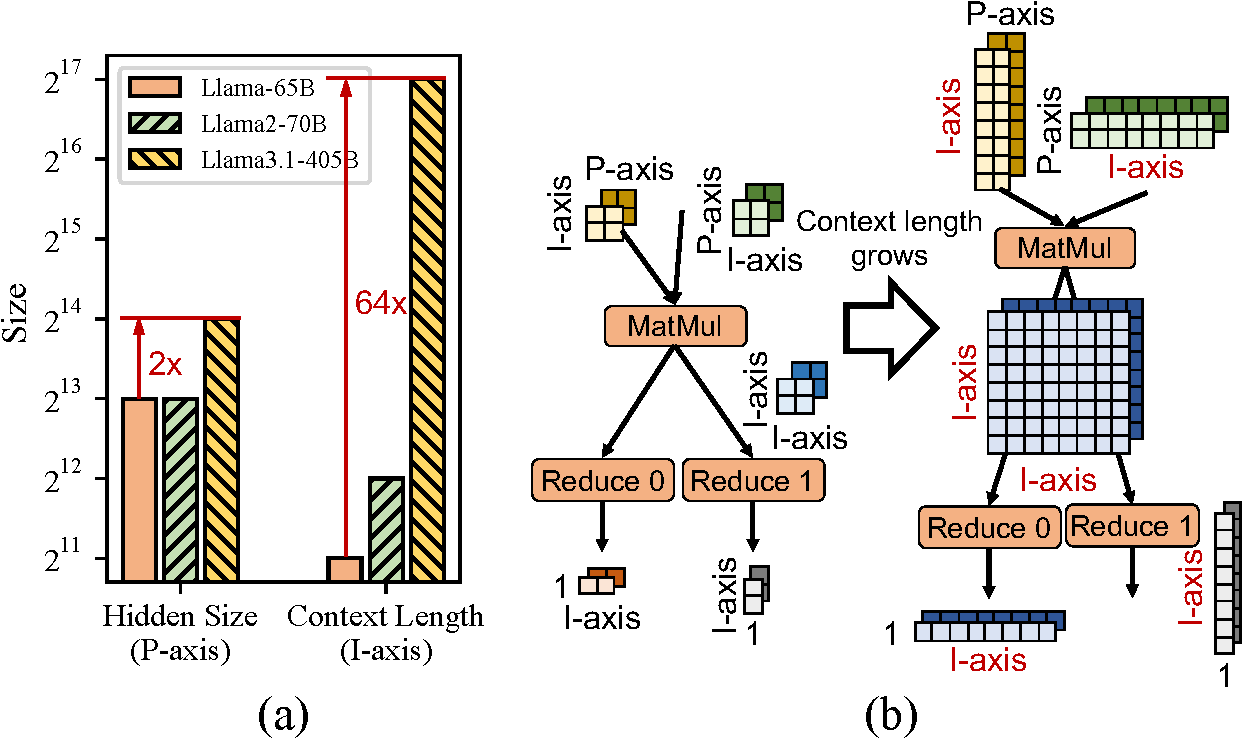
\includegraphics[width=0.85\linewidth]{figures/flashtensor/intro_workload-crop.pdf}
    % \vspace{-2em}
    \caption{模型张量增长情况与注意力变体示例}
    % \vspace{-1.5em}
    \label{fig:flashtensor-larger_workload}
\end{figure}

经调研总结,本文发现这两个方面的增长速度存在明显差异。
例如,从 Llama-65B 到 Llama-3.1-405B~\cite{touvron2023llama, touvron2023llama2, dubey2024llama3},P维度(隐藏层大小)从 8k 增加到 16k,仅增长了 2 倍;
而 I 维度(上下文长度)从 2k 扩展到 128k,增长了 64 倍,如\Cref{fig:flashtensor-larger_workload}(a)所示。
不同轴的增长速度差异导致模型中间张量的大小与形状出现显著变化。
\Cref{fig:flashtensor-larger_workload}(b)展示了注意力变体的一个简化部分计算图,其中包含一个矩阵乘法(MatMul)操作,
随后是两个不同归约方向的归约(Reduce)操作。
当 P 维度和 I 维度的大小相近时,MatMul 操作的输入和输出形状相似;
但在当前 P 维度和 I 维度大小差异巨大的情况下,MatMul 的输出相比计算中涉及的其他张量变得极其庞大。
这些巨大的张量需要耗费大量的处理时间,其计算效率对整体性能至关重要。

然而,由于算子操作的复杂性,当前的方法~\cite{tensorrt, torchcompile, zheng2023einnet, chen2018tvm, hu2024korch}在优化这些巨大张量时往往不能提供有效的解决方案。
如\Cref{fig:flashtensor-larger_workload}(b)所示,MatMul 的输出张量极大,融合是消除该张量并减少内存开销的有效方法之一。
但该张量随后被两个 Reduce 算子使用,一个按行归约,另一个按列归约。
如果进行融合,两个 Reduce 算子因不同归约维度导致的复杂依赖关系会降低并行性,大幅降低性能。
了解流经计算图边的中间张量的属性,如上述对特定轴的归约依赖,对于找到算子图的高效解决方案至关重要,更多有用的张量属性类型将在后文讨论。

在现有工作中,一方面,手动开发与优化算子库的研究~\cite{dao2022flashattention, dao2023flashattention, shah2024flashattention, ye2025flashinfer}虽然能够带来相对极致的性能,但无法涵盖层出不穷的众多新型模型结构变体。
另一方面,深度学习编译器~\cite{niu2021dnnfusion, astitch, shi2023welder}具备自动优化能力,但大多考虑张量大小、算子类型等相对粗粒度张量属性,往往忽略归约方向等细粒度张量属性,丢失了针对长序列场景下的深度优化机会。

本研究提出了 FlashTensor,通过利用细粒度张量属性来优化长序列后训练场景下的算子性能。
经研究观察,许多张量属性对于分析和优化以实现最佳性能至关重要,例如归约依赖、广播方向、大小和值等属性。
基于这一观察,FlashTensor 定义了张量的一些关键属性,并在计算图中识别它们,然后通过张量属性感知变换和内核映射策略优化张量程序。
本研究在 7 个模型上进行的实验,实验结果表明,与最先进的深度学习编译器相比,FlashTensor 的端到端加速比平均达到 1.50 倍,核心模块加速比平均达到 3.24 倍。
本章研究的主要贡献如下:

1. 总结了四个关键的细粒度张量属性,并设计了张量属性识别器,用于系统地分析整个计算图并捕获每个张量的属性。

2. 提出了细粒度张量属性感知的编译优化方法,基于属性感知变换规则和内核映射策略搜索最优内核,以实现高计算效率和低内存访问开销。

3. 基于上述设计实现了一个利用细粒度张量属性优化张量算子性能的系统 FlashTensor,其性能优于当前最先进的系统。

\begin{figure}[ht]
    \centering
    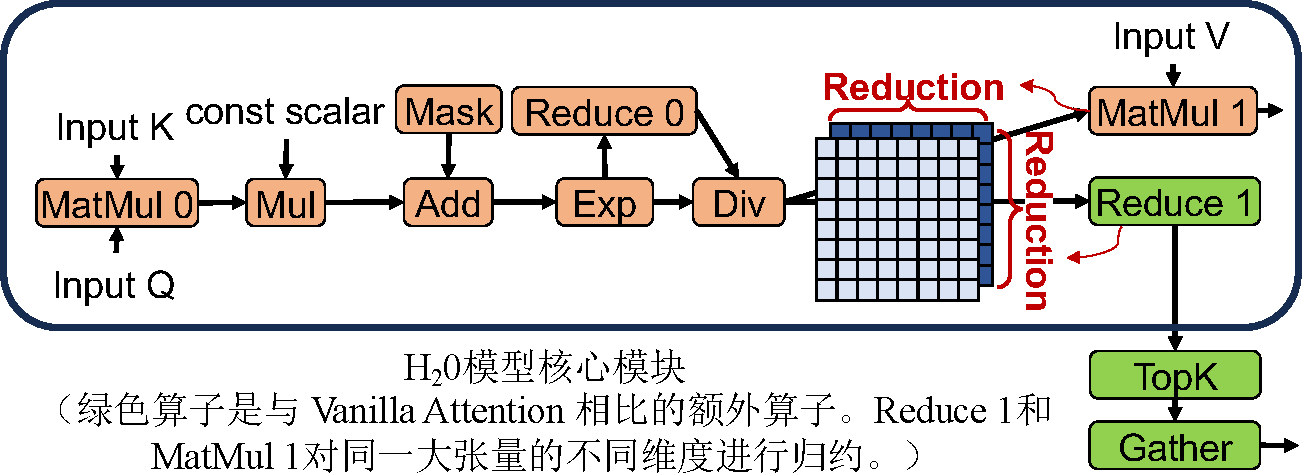
\includegraphics[width=0.7\linewidth]{figures/flashtensor/motivation_example_h2o_overview-crop.pdf}
    % \vspace{-1.7em}
    \caption{\(H_{2}O\) 模型示例}
    % \vspace{-2em}
    \label{fig:flashtensor-motivation_example_h2o_overview}
\end{figure}

\section{研究动机}

在大语言模型中,注意力机制是核心组件之一,负责捕捉输入序列中词元之间的依赖关系。
然而,传统的注意力机制在处理长上下文时会产生巨大的内存开销和计算量,尤其是在输入序列长度显著增加时。
在模型算法测,近期的一个研究热点是使用新的注意力变体来减少传统注意力机制的大量计算。
例如,\(H_{2}O\)~\cite{zhang2024h2o}、RoCo~\cite{ren2024roco} 和 Keyformer~\cite{adnan2024keyformer} 等模型可以丢弃一些不重要词元的数据以减少总计算量。
以\(H_{2}O\)为例(见\Cref{fig:flashtensor-motivation_example_h2o_overview}),它在 SoftMax(由 Exp、Reduce 0 和 Div 组成)之后使用一个额外的 Reduce 算子(Reduce 1)来计算词元的重要性,然后通过 TopK 算子结合 Gather 算子,选择并缓存最重要的词元数据,同时丢弃其余词元数据。

\(H_{2}O\)在后训练的推理过程时,包括两个阶段:预填充阶段(Prefill)和解码阶段(Decode)。
在预填充阶段,输入提示会被逐块处理,重要的词元会被选择并缓存数据,特别是当输入超过缓存容量时;
在解码阶段,输出词元数据会依次生成,并且在选择和保留最重要的词元数据时,缓存会进一步更新。
因此,新增的算子会影响预填充阶段和解码阶段的性能。
然而,对于长上下文文档摘要等任务,预填充阶段成为显著的性能瓶颈。
例如,在 InfiniteBench~\cite{zhang2024infinitebench} 中,提示的词元数可达 442K,而生成的词元数仅为 0.7K,相差 631 倍,导致\(H_{2}O\)中预填充与解码的执行时间比达到 4.51。
主要瓶颈源于预填充阶段核心模块中创建的大张量(见\Cref{fig:flashtensor-motivation_example_h2o_overview}),该张量由 MatMul 0 产生,大小为\(O(seqlen ^{2})\),导致大量的内存访问开销。
即使经过 TensorRT~\cite{tensorrt} 优化,\(H_{2}O\)的核心模块仍约占预填充总时间的 57.62\%,但计算性能仅达到 10.77 TFLOP/s(仅为 A100 F16 TensorCore 峰值性能的 3.45\%)。

关键挑战在于 MatMul 1 和 Reduce 1 这两个归约操作,它们对 Div 的输出张量(DivOut)具有不同的归约维度。为了提高效率,DivOut 的每一行必须分配到相同的并行单元用于 MatMul 1 操作,每一列也必须位于单个并行单元内。因此,除了使用单个并行单元外,没有其他可行的 DivOut 分区策略能满足这些约束。结果,像 TensorRT 这样的现有方法必须通过缓慢的全局内存跨多个内核处理大张量。此外,这两个具有不同归约维度的归约算子是\(H_{2}O\)与传统注意力机制的主要区别,由于这些结构差异,FlashAttention~\cite{dao2023flashattention} 难以对\(H_{2}O\)进行优化,其局限性源于缺乏对细粒度张量属性(如每个维度的归约依赖)的感知,从而错失了将 MatMul 1 与之前算子融合以避免访问大张量的机会。

\section{系统概述}

本研究通过利用细粒度张量属性来发掘更多算子融合机会,从而减少内存开销,提升推理运算性能。本节首先阐述对关键张量属性的观察,然后介绍FlashTensor系统设计。

\subsection{观察}

本小节列出一些细粒度的张量属性,并以\(H_{2}O\)模型为例说明它们为何对于发掘更多算子融合机会很重要。

\begin{itemize}

\item 
\textbf{归约依赖}:归约依赖指的是张量的某些维度是否会被聚合或归约,这对于分析算子的潜在并行机会至关重要。
如前所述,在\Cref{fig:flashtensor-motivation_example_h2o_overview}中,Div 的输出张量存在两个方向的归约依赖。
Reduce 1 无法在行维度上进行跨流式多处理器(SM)并行化,MatMul 1 无法在列维度上并行化,这使得整个计算图难以并行化。
识别这种归约依赖对于避免次优的并行化模式并寻找最优策略至关重要。
\item
\textbf{广播}:广播是指张量的维度被扩展或广播以匹配另一个张量的形状。
例如,\Cref{fig:dependency_and_broadcast_example}中的 Mul 算子隐式地对其右侧操作数的列维度进行广播。
何时进行广播对总计算量很敏感,图中示例里,重新排序后乘法计算量从\(NNh\)减少到\(Ndh\)。
但这种重新排序并不总是能得到正确结果,验证此类变换需要深入分析归约轴和广播轴之间的关系,这将后文进一步讨论。
\item
\textbf{大小}:大小是张量的固有属性,表示其包含的元素总数,与内存访问量密切相关,减少内存访问开销的关键策略之一就是最小化张量大小。
\item
\textbf{值}:值属性有助于减少不必要的计算和内存访问。例如,当了解到解码器-Transformer 中常用的三角掩码以及其上算子的含义后,可以跳过大多数张量中一半的计算。

\end{itemize}

\begin{figure}[htbp]
    \centering
    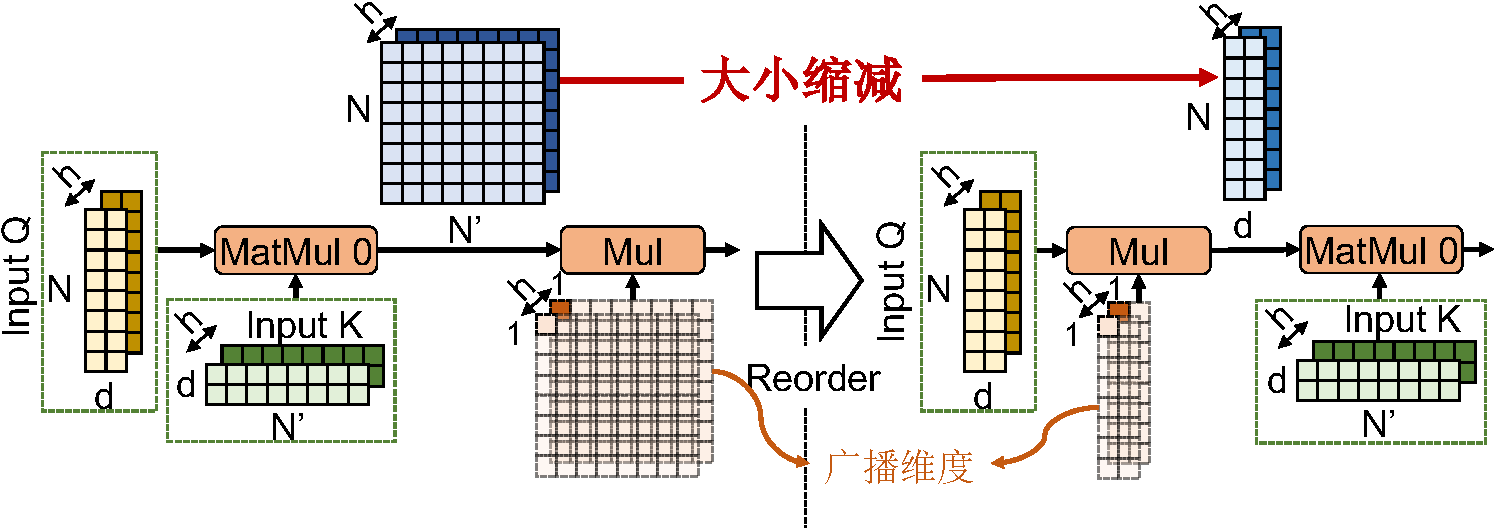
\includegraphics[width=0.7\linewidth]{figures/flashtensor/motivation_example_dependency_and_value-crop.pdf}
    % \vspace{-2em}
    \caption{\(H_{2}O\)模型中的广播示例}
    % \vspace{-1.7em}
    \label{fig:dependency_and_broadcast_example}
\end{figure}

\subsection{FlashTensor 系统设计}
基于上述观察,本研究提出了考虑这些细粒度张量属性的 FlashTensor。
如研究动机部分所述,FlashTensor 专注于优化长上下文任务的瓶颈——预填充阶段。
\Cref{fig:flashtensor-overview}展示了 FlashTensor 的总体架构,它主要由两个模块组成:张量属性识别器和张量属性感知优化器。
首先,张量属性识别器模块将张量程序作为输入(以计算图表示,节点表示算子,边表示张量),并捕获计算图中每个张量的所有细粒度属性,包括归约依赖、广播、大小和值。
然后,张量属性感知优化器模块根据图变换规则和内核映射策略搜索最优方案。
图变换规则旨在在特定限制下减小中间张量的大小,内核映射策略则通过考虑内存访问、计算强度和并行性来寻找高效的候选内核。
最终生成优化后的张量程序,可作为高效代码执行。

\begin{figure}[ht]
    \centering
    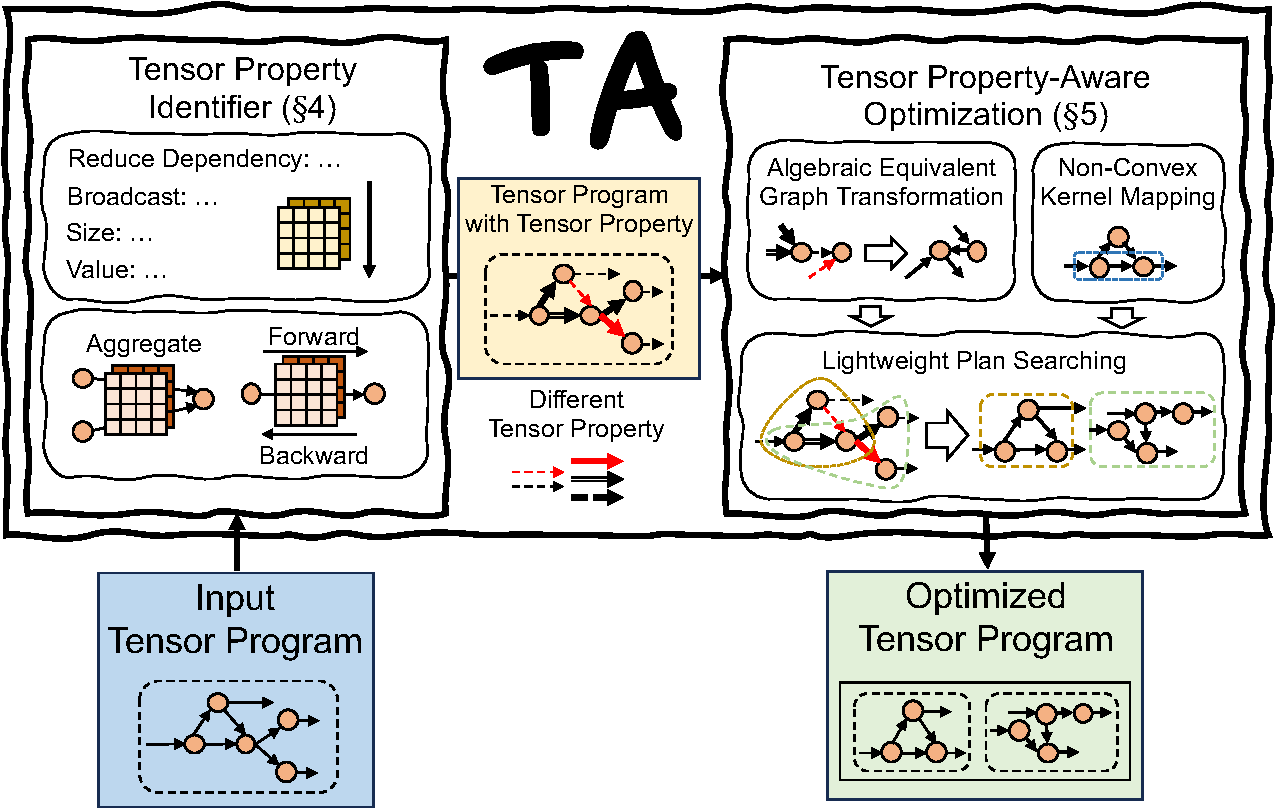
\includegraphics[width=0.7\linewidth]{figures/flashtensor/overview-crop.pdf}
    % \vspace{-1.5em}
    \caption{FlashTensor系统设计}
    % \vspace{-2em}
    \label{fig:flashtensor-overview}
\end{figure}



\section{张量属性识别器}
本节首先正式定义对后续分析和优化至关重要的张量属性,然后介绍 FlashTensor 如何在计算图中识别这些属性。



\subsection{属性定义}
如\Cref{tab:property}所示,张量属性分为两个不同类别:
1){逐维属性}:张量单个维度的特定属性,提供有关归约依赖和广播能力等方面的信息;
2){整体张量属性}:涵盖描述整个张量的属性,如总大小和可能的常数值。

\begin{table}[ht]
\centering
% \footnotesize
\caption{FlashTensor中的张量属性}
% \vspace{-0.5em}
\begin{tabular}{p{1.4cm}<{\centering}cp{4.2cm}}
\toprule
\multicolumn{3}{c}{\textbf{逐维度属性}} \\

\hline
\multirow{3}{*}{\makecell{归约\\依赖}} & \multirow{1}{*}{\makecell{NonPara}} & 不可并行化维度 \\
                             & \multirow{1}{*}{\makecell{Batch}} & 完全可并行化维度 \\
                             & \multirow{1}{*}{\makecell{Reuse}} & 具有数据复用的可并行化维度 \\
\hline

\multirow{2}{*}{\makecell{广播}} & No & 未广播维度 \\
                           & Yes & 已广播维度 \\
\hline
\multicolumn{3}{c}{\textbf{整体张量属性}} \\
\hline
\makecell{大小} & 整数 & 张量的总大小 \\
\hline
\multirow{7}{*}{\makecell{值}} & Var & 张量值未确定 \\
                       & Zero & 全零张量 \\
                       & PosConst & 正常量张量 \\
                       & NegConst & 负常量张量 \\
                       & PosInf & 正无穷大张量 \\
                       & NegInf & 负无穷大张量 \\
                       & NaN & 非数值张量 \\
\bottomrule
\end{tabular}
% \vspace{-1.0em}
\label{tab:property}
\end{table}


\begin{itemize}
\item
\textbf{归约依赖}:归约依赖属性是一个多值属性,描述张量维度与归约操作之间的相互依赖关系,这对优化计算效率至关重要。
它有三个取值:
1) NonPara:表示由于归约操作的数据依赖,无法进行并行执行分区的维度。这些维度需要由单个单元处理,无法并行化。例如,在\Cref{fig:property_definition_dependency}(a)中,输入和输出的归约维度都被归类为 NonPara,因为它们需要在整个维度上进行数据聚合。
2) Reuse:表示可以并行化且能通过分块实现数据重用的维度。例如,在\Cref{fig:property_definition_dependency}(b)中,MatMul 的行维度可以并行化,通过分块重用右侧操作数可提高内存效率,这种方法也适用于支持广播的操作,如 Add 和 Mul,分块后并行化可平衡计算效率和内存访问。
3) Batch:表示可以完全并行化且无需数据重用的维度,如\Cref{fig:property_definition_dependency}(b)中批量矩阵乘法的批次维度,以及\Cref{fig:property_definition_dependency}(a)中 Reduce 操作除归约维度外的其他维度。

\begin{figure}[ht]
    \centering
    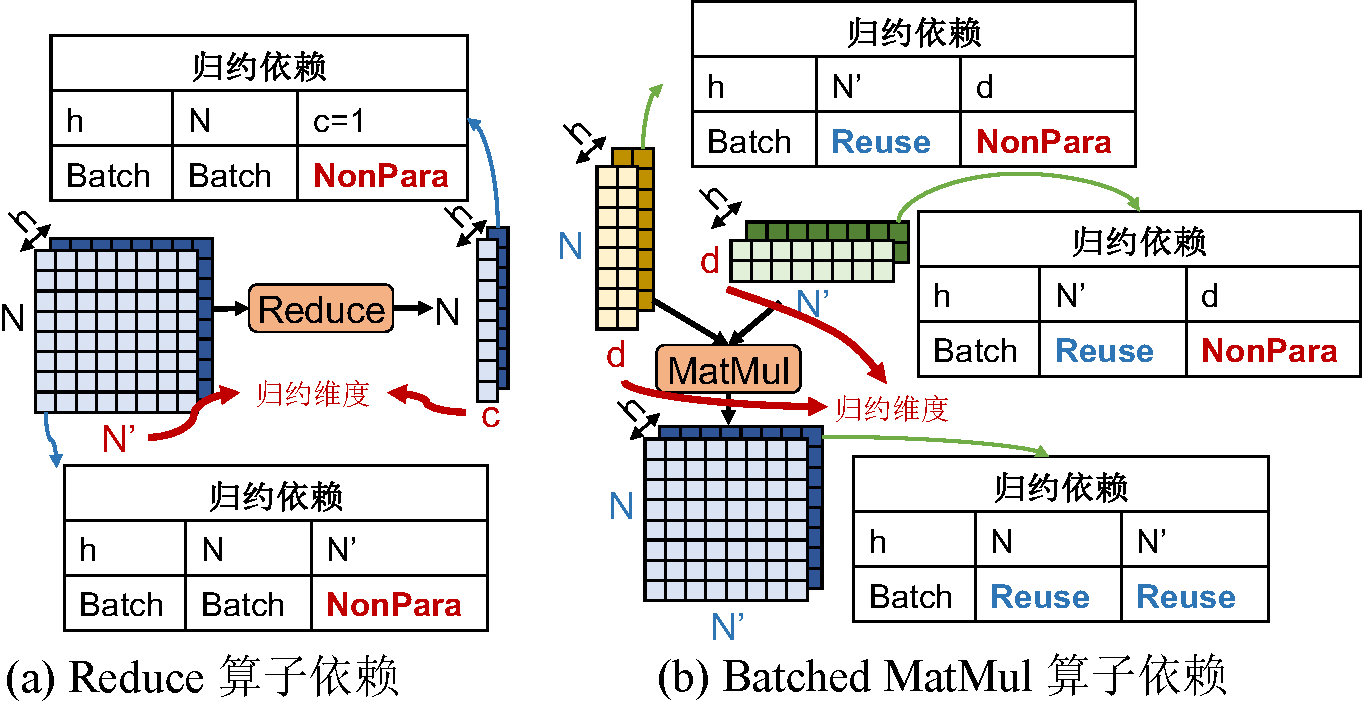
\includegraphics[width=0.7\linewidth]{figures/flashtensor/property_definition_dependency-crop.pdf}
    % \vspace{-1.9em}
    \caption{归约依赖属性}
    % \vspace{-1.5em}
    \label{fig:property_definition_dependency}
\end{figure}

\item
\textbf{广播}:该属性表示张量的某个维度是否会被后续算子广播。如果张量在某维度上是支持广播算子的操作数,则该维度被视为广播维度。\Cref{fig:property_definition_broadcast}(a)(b)展示了维度如何扩展以满足算子形状要求的示例。
\item
\begin{figure}[ht]
    \centering
    % \includegraphics[width=0.93\linewidth]{figures/property_definition_broadcast-crop.pdf}
    \includegraphics[width=0.65\linewidth]{figures/flashtensor/property_definition_broadcast-crop.pdf}
    % \vspace{-1em}
    \caption{广播属性}
    % \vspace{-1.5em}
    \label{fig:property_definition_broadcast}
\end{figure}

\textbf{大小}:表示张量中元素的总数,计算为所有维度的乘积,如\Cref{fig:property_definition_size_and_value}所示。
\item
\textbf{值}:指示张量在计算过程中是否保持常数值,如\Cref{fig:property_definition_size_and_value}所示。
与传统编译器将常量视为标量不同,FlashTensor 在张量级别处理常量,从而提供更广泛的优化机会。
具有常数值的张量可以预先计算或高效存储,减少执行期间的动态更新。
在 FlashTensor 中,常数值信息以枚举形式表示,而非实际值,以平衡信息有效性和开销。
\end{itemize}





\begin{figure}[htbp]
    \centering
    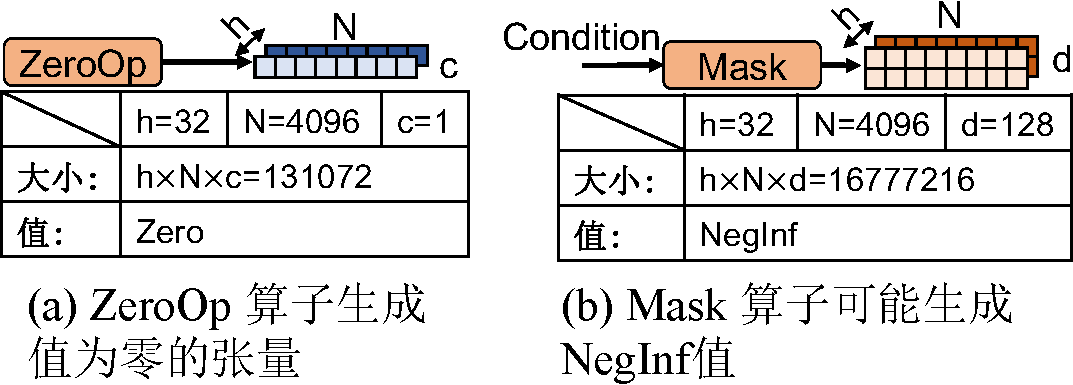
\includegraphics[width=0.52\linewidth]{figures/flashtensor/property_definition_size_and_value-crop.pdf}
    % \vspace{-0.7em}
    \caption{大小和值属性}
    % \vspace{-2em}
    \label{fig:property_definition_size_and_value}
\end{figure}



% \begin{table}[h]
% \footnotesize
% \caption{Tensor properties in FlashTensor. The second column lists the potential values for each corresponding property.}
% % \vspace{-0.5em}
% \begin{tabular}{|p{1.4cm}<{\centering}|c|p{4.2cm}|}
% \hline
% \multicolumn{3}{|l|}{\textbf{Per-Dimension Property}} \\

% \hline
% \multirow{3}{*}{\makecell{Reduce\\dependency}} & \multirow{1}{*}{\makecell{NonPara}} & Non-parallelizable dim. \\
%                              & \multirow{1}{*}{\makecell{Batch}} & Embarrassingly parallelizable dim. \\
%                              & \multirow{1}{*}{\makecell{Reuse}} & Parallelizable dim with data reuse. \\
% \hline

% \multirow{2}{*}{\makecell{Broadcast}} & No & Unbroadcasted dim. \\
%                            & Yes & Broadcasted dim. \\
% \hline
% \multicolumn{3}{|l|}{\textbf{Entire Tensor Property}} \\
% \hline
% \makecell{Size} & An integer & The total size of the tensor. \\
% \hline
% \multirow{7}{*}{\makecell{Value}} & Var & The tensor value is undetermined. \\
%                        & Zero & The tensor is all zero. \\
%                        & PosConst & The tensor is a positive constant. \\
%                        & NegConst & The tensor is a negative constant. \\
%                        & PosInf & The tensor is positive infinity. \\
%                        & NegInf & The tensor is negative infinity. \\
%                        & NaN & The tensor is not a number. \\
% \hline
% \end{tabular}
% % \vspace{-1.0em}
% \label{tab:property}
% \end{table}

\subsection{基于数据流的属性识别}
一些基本属性(如大小)可以很容易地从张量中提取,但像归约依赖这样的复杂属性则需要复杂的分析才能准确标注。
例如,在单个算子中,即使不完全实现算子,也可以根据其计算语义简单标注输入和输出张量的归约依赖,如\Cref{fig:property_definition_dependency}所示。
然而,在包含多个算子的计算图中,张量的归约依赖属性会受到后续和前面算子的影响,难以确定其确切值。

为解决这个问题,本研究提出了一种基于两阶段数据流的属性识别算法:
1) \textbf{属性传播}:根据每个算子的计算语义,张量属性进行前向和后向传播。
2) \textbf{属性聚合}:将从各个算子传播来的属性进行聚合,以确定每个张量的最终属性值。
该算法利用固有的单调优先级(例如,归约依赖类型:NonPara > Reuse > Batch)。
当不同类型的属性在同一张量维度上汇聚时,保留优先级较高的值,以确保在整个图中准确表示属性。
这些阶段会迭代执行,直到属性稳定。
\Cref{fig:identification_merge}给出了归约依赖识别的示例以进一步说明。\Cref{fig:identification_merge}(b)展示了 MatMul 的输出如何通过后向传播将右侧操作数在 N’维度上的归约依赖从 Reuse 更新为 NonPara;\Cref{fig:identification_merge}(a)展示了 MatMul 和 Reduce 之间的属性聚合过程,中间张量从两个算子接收不同的归约依赖值。

\begin{figure}[ht]
    \centering
    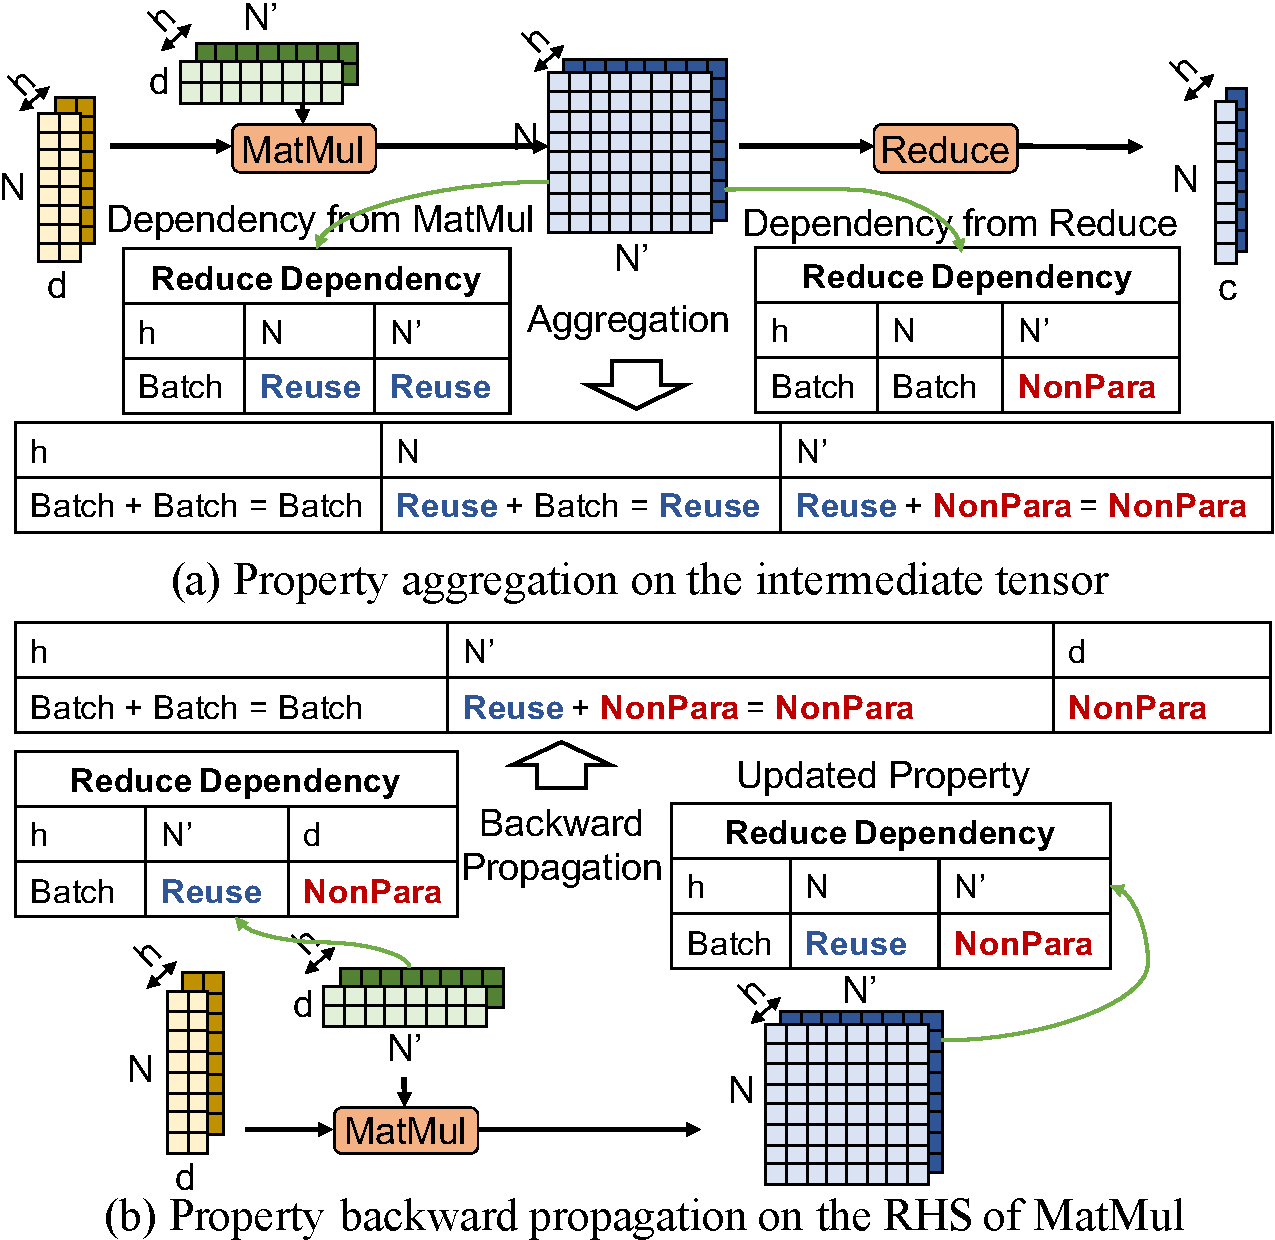
\includegraphics[width=0.7\linewidth]{figures/flashtensor/identification_merge-crop.pdf}
    % \vspace{-1.5em}
    \caption{归约依赖属性识别示例}
    % \vspace{-1em}
    \label{fig:identification_merge}
\end{figure}

\section{细粒度张量属性感知优化}
FlashTensor 基于识别出的细粒度张量属性进一步优化张量程序。
优化基于两个规则(代数等价图变换和非凸内核映射)以及一种轻量级方案搜索方法。
代数等价图变换提供一系列变换规则,允许通过等价变换改变中间张量的大小;
非凸内核映射提出一种新的候选内核以实现高效执行;
轻量级方案搜索通过属性约束剪枝和低成本性能模型实现高效的方案生成。

\subsection{代数等价图变换}
中间张量的大小是决定内存访问开销的主要因素。
因此,本研究提出一种变换方法,主要通过对计算图进行代数等价变换来关注中间张量大小的变化,这使得后续能够在整个搜索空间中寻找中间张量大小最小的计算图,从而减少内存开销。
{广播是导致中间张量大小变化的本质原因}。


\begin{table}[ht]
    \centering
    \caption{基于广播属性的转换规则}
    % \vspace{-0.5em}
    % \footnotesize
    \begin{tabular}{ccc}
       \toprule
       规则  & 注释 & 条件 \\
       \hline
       $A + B = B + A$  & 交换律 & 否 \\  
       $A \odot B = B \odot A$  & 交换律 & 否 \\  
       
       $A + (B + C) = (A + B) + C$  & 结合律 & 否 \\  
       $A \odot (B \odot C) = (A \odot B) \odot C$  & 结合律 & 否 \\  
       $\sum_i(A + B) = \sum_iA + \sum_iB$ & 结合律 & 否 \\

       $A \odot C + B \odot C = (A + B) \odot C$ & 分配律 & 否 \\
       $A / C + B / C = (A + B) / C$ & 分配律 & 否 \\

        \hline

       $\sum_i(A \odot B) = (\sum_iA) \odot (\sum_iB)$ & 分配律 & 是 \\
       \multicolumn{3}{r}{若 $A \odot B$ 中 $A$ 或 $B$ 在维度 $i$ 上被广播} \\
       
       $\sum_i(A / B) = (\sum_iA) / (\sum_iB)$ & 分配律 & 是 \\
       \multicolumn{3}{r}{若 $A / B$ 中 $B$ 在维度 $i$ 上被广播} \\
       
       $(A \odot B)C = (AC) \odot B$ & 分配律 & 是 \\
       \multicolumn{3}{r}{若 $B$ 在 $AC$ 的归约维度上被广播} \\
       
       $(A / B)C = (AC) / B$ & 分配律 & 是 \\
       \multicolumn{3}{r}{若 $B$ 在 $AC$ 的归约维度上被广播} \\
       \bottomrule
    \end{tabular}
    % \vspace{-1.5em}
    \label{tab:broadcast_based_transform}
\end{table}




(1) \textbf{基于广播属性的变换规则}:本研究提出了一系列变换规则,这些规则不仅考虑张量大小,还考虑每个维度的广播属性。具体而言,\Cref{tab:broadcast_based_transform}列出了所有变换规则。$A$、$B$ 和 $C$ 为张量。$+$、$\odot$ 和 $/$ 分别为逐元素加、乘和除。$AB$ 表示 $A$ 和 $B$ 的矩阵乘法。除矩阵乘法外的所有运算符均支持广播。主要规则可分为两大部分:
始终有效的变换:无论操作数的广播属性如何,这些变换始终有效,其有效性由不同算子及其组合的交换律、结合律和分配律这三个数学定律保证。

\begin{figure}[ht]
    \centering
    % \includegraphics[width=0.8\linewidth]{figures/wo_broadcast-crop.pdf}
    \includegraphics[width=0.75\linewidth]{figures/flashtensor/wo_broadcast-crop.pdf}
    % \vspace{-0.7em}
    \caption{MatMul 与 Div 算子重排序示例}
    % \vspace{-1.3em}
    \label{fig:wo_broadcast}
\end{figure}

(2) \textbf{受广播属性约束的变换}:某些变换的有效性取决于广播属性。在这些变换中,广播被视为确保正确性的关键属性。例如,在\Cref{fig:wo_broadcast}(a)中,当 Div 的右侧操作数在 N 维度上广播时,重新排序是无效的,因为 MatMul 中的归约会破坏计算语义,导致结果错误;而在\Cref{fig:wo_broadcast}(b)中,如果 Div 的右侧操作数沿与 MatMul 归约维度对齐的维度广播,重新排序则是有效的。

(3) \textbf{基于值属性的变换规则}:本研究利用值属性通过消除不必要的迭代来优化循环。具体而言,重点是在不影响最终输出的情况下跳过 For 循环中的某些迭代。如\Cref{fig:value_example}所示,某些迭代可能会从 Mask 算子产生常量值(如 -∞),由于这些常量值在 For 循环中保持不变地传播,FlashTensor可以识别并安全地跳过这些迭代,这不仅保持了输出的正确性,还减少了计算量。

\begin{figure}[ht]
    \centering
    % \vspace{-1em}
    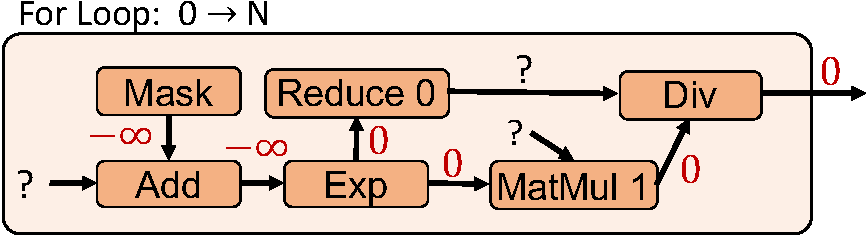
\includegraphics[width=0.5\linewidth]{figures/flashtensor/value_example-crop.pdf}
    % \vspace{-1em}
    \caption{值属性示例}
    % \vspace{-1em}
    \label{fig:value_example}
\end{figure}


\subsection{非凸内核映射}
内核映射是指在现代硬件平台上将计算图中的算子分配给 GPU 内核执行。
对于给定的计算图,简单地将所有算子融合到单个内核中,由于复杂的归约依赖和有限的并行性,往往会导致性能不佳,因此识别合适的内核以实现高效执行至关重要。

首先,本文给出最先进研究中内核的形式化定义。

\vspace{0.5em}
\begin{definition}[内核] 对于计算图\(G=(V, E)\),如果不存在节点\(p_{1}, p_{2} \in K\)和另一个节点\(q \in V/K\),使得\(p_{1} \stackrel{G}{\rightsquigarrow } q\)且\(q \stackrel{G}{\rightsquigarrow} p_{2}\)(其中\(x \stackrel{G}{\rightsquigarrow} y\)表示在\(G\)中存在从\(x\)到\(y\)的路径),则节点集\(K \subseteq V\)构成一个内核。
\end{definition}
\vspace{0.5em}

该定义将计算图中的凸子集算子视为内核,凸性意味着这种内核不能包含通过外部算子依赖自身的算子,如\Cref{fig:kernel_def_diff}(a)所示。
Korch~\cite{hu2024korch} 认为由于循环依赖(即 Div 依赖于 Reduce,Reduce 又依赖于 Exp),这样的内核无法执行,但这种循环依赖可以通过其他内核解决,具体而言,一个内核不必生成自身输入,只要有其他内核提供这些输入即可。
例如,为解决\Cref{fig:kernel_def_diff}(a)中的循环依赖,包含 Exp 和 Reduce 的另一个内核可以提供输入,从而使包含 Div 的内核能够顺利执行。基于这一理解,本研究放宽了传统内核定义的限制,提出了非凸内核的概念。

\vspace{0.5em}
\begin{definition}[非凸内核] 对于计算图\(G=(V, E)\),当且仅当存在一个存在节点\(p_{1}, p_{2} \in K\)和另一个节点\(q \in V/K\),使得\(p_{1} \stackrel{G}{\rightsquigarrow } q\)且\(q \stackrel{G}{\rightsquigarrow} p_{2}\),节点集\(K \subseteq V\)构成一个非凸内核。
\end{definition}
\vspace{0.5em}

非凸内核的引入为算子的分配提供了更大的灵活性,有助于更好地适应复杂的计算图结构。
在确定内核时,本研究考虑了计算强度、内存访问模式和并行性等因素。
计算强度较高的算子倾向于被组合在一起,以充分利用硬件的计算资源。
同时,尽量减少内核之间的数据传输,以降低内存访问开销。
例如,对于具有相似内存访问模式的算子,将它们映射到同一个内核中,可以减少内存访问的次数和延迟。

\begin{figure}[ht]
    \centering
    % 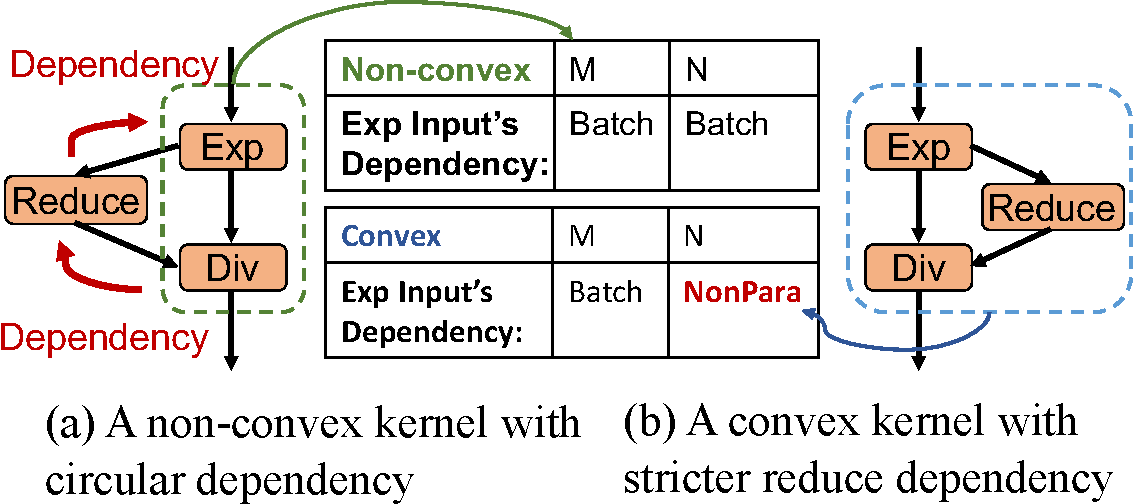
\includegraphics[width=0.85\linewidth]{figures/kernel_def_diff-crop.pdf}
    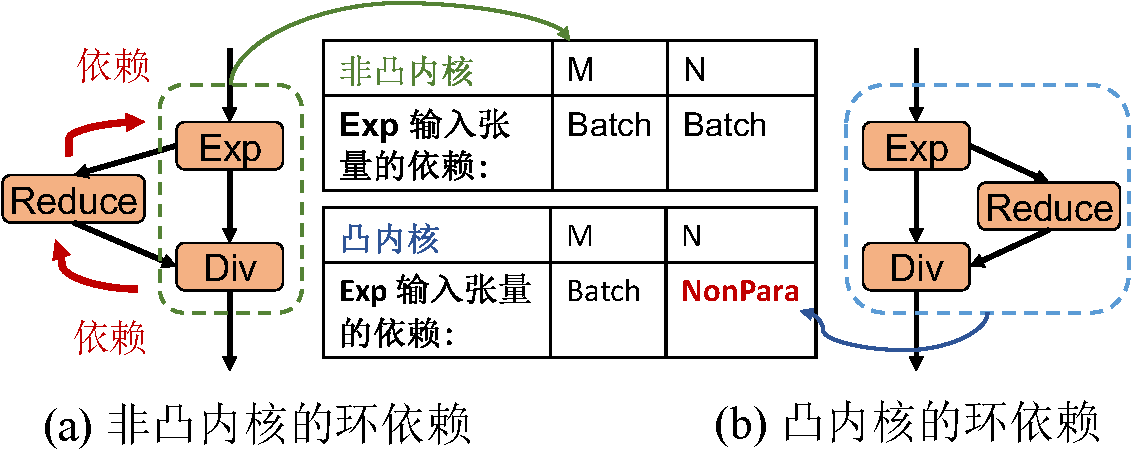
\includegraphics[width=0.6\linewidth]{figures/flashtensor/kernel_identification-crop.pdf}
    % \vspace{-0.8em}
    \caption{非凸内核与凸内核示例}
    % \vspace{-1.5em}
    \label{fig:kernel_def_diff}
\end{figure}


\subsection{轻量级方案搜索}
为了找到最优的内核映射方案,本研究采用了一种基于搜索的方法。该方法从一个初始的内核映射方案出发,通过对算子的分配进行小的调整,生成一系列候选方案。对于每个候选方案,本研究评估其性能,包括计算时间、内存使用量等指标。评估过程使用了一个轻量级的性能模型,该模型基于硬件的特性和算子的属性,能够快速估算出不同方案的性能表现。通过不断迭代搜索过程,逐步找到性能最优的内核映射方案。

在搜索最优的计算图变换和内核映射方案时,由于可能的方案数量庞大,穷举搜索是不可行的。因此,本研究提出了一种轻量级的方案搜索方法,该方法结合了属性约束剪枝和低成本性能模型,以高效地生成有潜力的方案。

(1) \textbf{属性约束剪枝}:本研究利用在张量属性识别阶段得到的张量属性信息,对搜索空间进行剪枝。
例如,如果一个张量的某个维度具有 NonPara 类型的归约依赖,那么在考虑并行化方案时,就可以排除那些涉及该维度并行化的方案,因为这些方案在实际执行中无法满足数据依赖要求,必然会导致性能不佳。
通过这种方式,能够显著减少需要评估的方案数量,提高搜索效率。

(2) \textbf{低成本性能模型}:为了快速评估不同方案的性能,本研究构建了一个低成本性能模型。
该模型考虑了算子的计算复杂度、内存访问开销以及硬件的特性。
例如,对于矩阵乘法算子,模型根据其输入矩阵的大小计算计算量;根据数据在内存中的存储布局和访问模式,估算内存访问时间。
通过将这些因素综合考虑,模型能够快速给出一个方案的性能估计值,允许在短时间内对大量候选方案进行评估和比较,从而筛选出有潜力的方案进行进一步优化。


整个搜索算法如\Cref {alg:kernel_identify}所示。
该算法首先确定可用的并行执行单元数量,例如 GPU SM的数量。
然后,遍历计算图的连通子集,筛选出并行度或算术强度低于性能阈值的内核。
在筛选出候选内核后,本研究遵循先前的工作~\cite{hu2024korch},将最优候选搜索形式化为一个二元线性规划任务并求解。

\begin{algorithm}[ht]
{
% \fontsize{8pt}{9pt}\selectfont
\caption{核识别}
    \label{alg:kernel_identify}
    % \small
    \SetAlgoNlRelativeSize{0}
    \SetAlgoNlRelativeSize{-1}
    \SetKwProg{Fn}{函数}{:}{}
    \KwData{计算图 $G$,算术强度阈值 $H$}
    \KwResult{$G$ 中的候选核 $K$}
    \Fn{搜索($G$)} { 
        $K = \emptyset $\; 
        最大并行单元数 $\leftarrow$ 查询底层加速器\;
        \ForEach{连通子集 $X$ $\in$ $G$}{
            $AI \leftarrow$ 计算 $X$ 的算术强度\;
            并行单元数 $\leftarrow$ 获取 $X$ 的并行度\;
            \If{$AI \geq H$ 且 并行单元数 $\geq$ 最大并行单元数}{
                $K = K \cup \{X\}$\;
            }
        }
        \Return $K$\;
    }
}
\end{algorithm}

\section{实验评估}
FlashTensor 基于 MLIR~\cite {lattner2020mlir} 和 Triton~\cite {tillet2019triton},由 10K 行 C++ 代码和 2K 行 Python 代码实现。
FlashTensor 以 ONNX 格式(可通过现有工具从原生 TensorFlow/PyTorch 程序轻松导出)为输入,并将其转换为有效的 MLIR 代码。
本研究在 MLIR 中实现了两种方言:FT 和 FTTriton。
FT 定义了张量操作(如逐元素操作、归约、重塑和矩阵乘法)以及通过 MLIR passes 实现的相应转换;
FTTriton 作为从 FT 到 Triton DSL 的桥梁,定义了与 Triton 类似的操作符。
应用所有优化后,最终的 MLIR 代码将转换为有效的 Triton 代码,接入PyTorch算子后端。

\subsection{实验设置}
实验平台方面,本研究在配备 NVIDIA A100 和 H100 GPU 的服务器上进行实验,以评估 FlashTensor 的性能。
具体为:
1)一块 NVIDIA A100-PCIE-40GB GPU(配备两颗 AMD EPYC 7742 64 核 CPU);
2)一块 H100-PCIE-80GB GPU(配备 AMD EPYC 7453 28 核 CPU)。
软件版本为 Python 3.10、CUDA 12.1 和 GCC 12.2。

评估模型方面,实验选取了七个具有代表性的模型,包括\(H_{2}O\)~\cite{zhang2024h2o}, RoCo~\cite{ren2024roco}, Keyformer~\cite{adnan2024keyformer}, SnapKV~\cite{li2024snapkv}, Corm~\cite{dai2024corm}, Vanilla Attention~\cite{vaswani2017attention} (V.A.), Gemma2~\cite{team2024gemma2}等新型注意力变体模型,以及一些传统基于 Transformer 的模型。
这些模型涵盖了不同的应用场景和计算特点,能够全面地测试 FlashTensor 的优化效果。
这些模型的简要描述如~\Cref {tab:model_description} 所示。
在端到端实验中,所有模型均使用  {Llama-2-7b}~\cite {touvron2023llama2} 作为基础模型,采用 FP16 精度权重、32 个注意力头和 128 的头维度。为保证公平比较,模型间唯一差异在于注意力模块设计。


\begin{table}[ht]
    \centering
    % \footnotesize
    \caption{评估模型的基本信息}
    % \vspace{-1em}
    \begin{tabular}{lp{12cm}}
       \toprule
       模型   & 描述 \\
       \hline
       \(H_{2}O\)   & 它利用累积注意力分数来丢弃对最终注意力分数贡献较小的高频词元。 \\
       % \hline
       RoCo   & 它注意到注意力概率的标准差与词元重要性之间的关系,并利用这种关系来指导词元丢弃。 \\
       % \hline
       Keyformer  & 它使用基于 Gumbel 软最大化的分数函数来识别关键词元。 \\
       % \hline
       SnapKV   & 它利用聚类来保留重要词元的注意力特征。 \\
       % \hline
       Corm   & 它定义了长期次要键,并丢弃被视为长期次要键的词元。 \\
       % \hline
       V.A.   & 它是当前基于Transformer的模型中广泛使用的标准注意力机制。 \\
       % \hline
       Gemma2   & 它是一种新提出的模型,为注意力层引入了对数软上限。 \\
       \bottomrule
    \end{tabular}
    % \vspace{-1.5em}
    \label{tab:model_description}
\end{table}

对比系统方面,本研究将 FlashTensor 与八种最先进的深度学习优化方法进行对比。
1) {深度学习编译器}: PyTorch 2.2.2~\cite{pytorch19} and corresponding TorchInductor~\cite{torchcompile}, TensorRT 10.0.1~\cite{tensorrt},  TVM 0.16.0~\cite{chen2018tvm} with MetaScheduler~\cite{chen2018autotvm, zheng2020ansor}, Korch~\cite{hu2024korch}, 以及 EinNet~\cite{zheng2023einnet}. 
2) {高效算子库}: FlashAttention 2.6.2~\cite{dao2022flashattention, dao2023flashattention} 以及 FlashInfer 0.1.0~\cite{ye2025flashinfer}.

在实验过程中,本研究统一使用相同的数据集对所有模型进行推理测试,以确保实验结果的可比性。
对于每个模型,本研究分别测量其端到端的推理时间以及核心模块的执行时间,并计算性能加速比。
同时,本研究还记录了内存使用情况,以评估 FlashTensor 在减少内存开销方面的效果。

% \begin{figure*}[ht]
%     \centering
%     \begin{minipage}[ht]{\textwidth}
%         {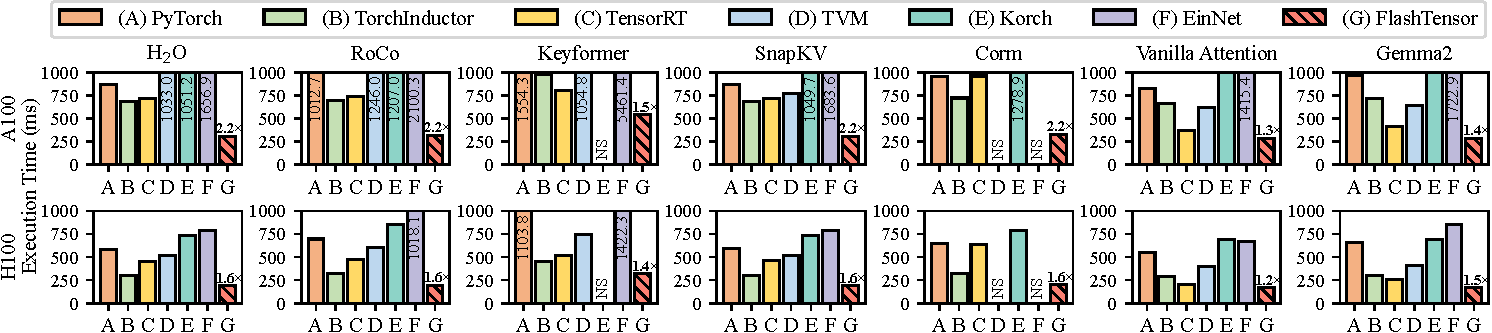
\includegraphics[width=\linewidth]{figures/flashtensor/e2e-crop.pdf}}
%         % \vspace{-1em}
%     \end{minipage}
%     \\
%     \centering \small (a) End-to-end performance
%     \begin{minipage}[ht]{\textwidth}
%         {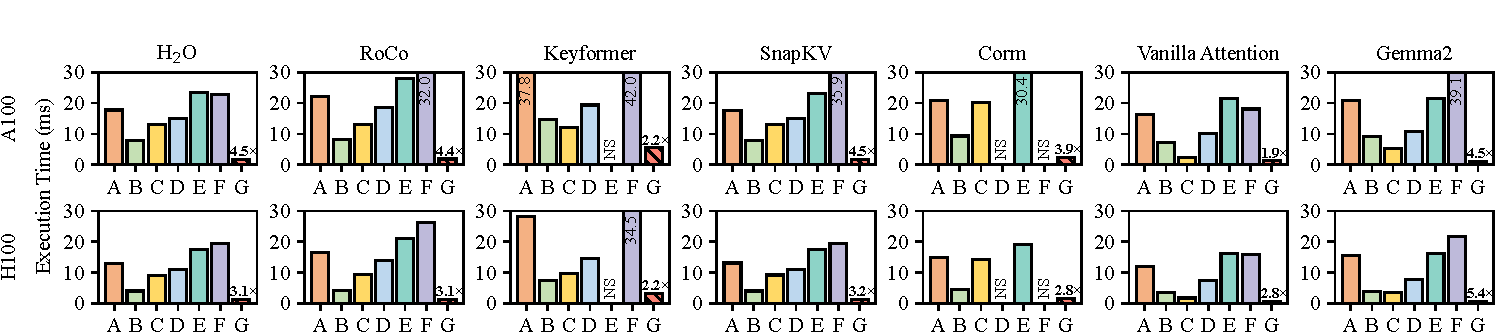
\includegraphics[width=\linewidth]{figures/flashtensor/kernel-crop.pdf}}
%         % \vspace{-1em}
%     \end{minipage}
%     \\
%     \centering \small (b) Core module performance
%     % \vspace{-1em}
%     \caption{End-to-end and core module performance comparison of seven evaluated models with SOTA systems on A100 and H100 GPU. NS means NotSupport. Bars for baselines of too long running time are truncated, and their execution times are marked on the bars. The numbers above FlashTensor's bars show FlashTensor's speedups over the best baseline.}
%     % \vspace{-0.5em}
%     \label{fig:e2e-kernel}
% \end{figure*}

\begin{figure}[ht]
    \centering
    \begin{minipage}[t]{\textwidth}
        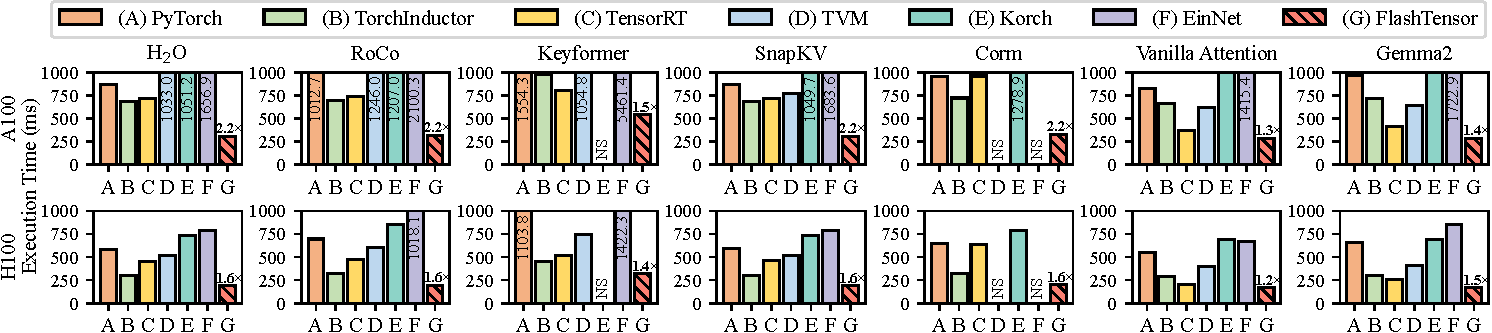
\includegraphics[width=\linewidth]{figures/flashtensor/e2e-crop.pdf}
    \end{minipage}
    \vspace{-0.5em}
    \caption*{\small (a) 端到端性能}
    
    \begin{minipage}[t]{\textwidth}
        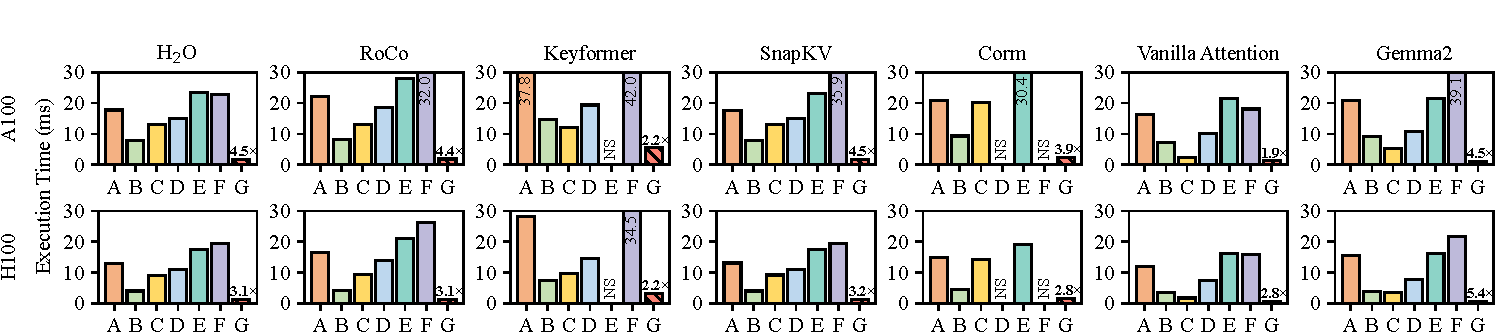
\includegraphics[width=\linewidth]{figures/flashtensor/kernel-crop.pdf}
    \end{minipage}
    \vspace{-0.5em}
    \caption*{\small (b) 核心模块性能}
    \caption{端到端和核心模块性能对比(A100和H100 GPU上)}
    \label{fig:e2e-kernel}
\end{figure}

\subsection{性能对比}

本研究首先比较了 FlashTensor 模型与最先进的深度学习编译器的端到端推理性能。
如\Cref {fig:e2e-kernel}所示,NS表示不支持,运行时间过长的基线柱状图被截断,其执行时间标注在柱状图上。
FlashTensor柱状图上方的数字显示了FlashTensor相对于最佳基线的加速比。

如\Cref {fig:e2e-kernel}(a) 所示,FlashTensor 在 A100 上的加速比最高可达最佳基线的\(2.22\times\),在 H100 上可达\(1.62\times\)。
FlashTensor 的性能提升主要来自高度优化的核心模块。
\Cref {fig:e2e-kernel}(b) 展示了核心模块(如注意力变体)的性能,FlashTensor 在 A100 上的加速比最高达\(4.52\times\),在 H100 上达\(5.43\times\)。

本研究观察到部分模型结构相似,在 FlashTensor 下性能大致相当,但经最先进的深度学习编译器优化后,性能差异显著。
例如,如~\Cref {fig:lib_cmp}(a) 所示,Gemma2 仅对标准注意力(V.A.)做了微小修改,绿色算子为 Gemma2 的额外结构。
使用 TensorRT 时,A100 上 Gemma2 和 V.A. 的推理时间分别为 5.13 和 2.25 毫秒——这种显著差距源于 TensorRT 针对 V.A. 的注意力结构预写了特定规则(类似 FlashAttention),但无法匹配 Gemma2 的微小修改结构。
而在 FlashTensor 中,A100 上 Gemma2 和 V.A. 的推理时间分别为 1.14 ms 和 1.20 ms,性能相当且超越 TensorRT。
这是因为 FlashTensor 通过张量属性感知规则自动搜索最优方案,既能适配不同模型,又能利用值感知循环迭代消除技术,进一步减少因果掩码导致的不必要计算。

\subsection{不同序列长度的可扩展性}
\Cref{fig:seqlen_mem_flops} 展示了 \(H_{2}O\) 在不同序列长度下的计算效率和内存占用可扩展性。  
\begin{figure}[ht]
    \centering
    % \vspace{-1.8em}
    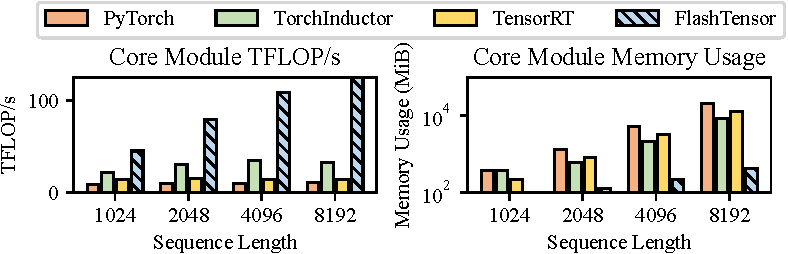
\includegraphics[width=0.7\linewidth]{figures/flashtensor/gflops_mem-crop.pdf}
    % \vspace{-1.7em}
    \caption{\(H_{2}O\) 在不同序列长度下的内存占用和 TFLOP/s}
    % \vspace{-0.5em}
    \label{fig:seqlen_mem_flops}
\end{figure}

计算效率方面,
每秒浮点运算次数(FLOP/s)是衡量内核计算效率或吞吐量的重要指标。
由于内存访问开销更低,FlashTensor 在序列长度较长时实现了更高的 FLOP/s。
TorchInductor 和 TensorRT 采用相同的内核映射策略,需在 CUDA 内核中从全局内存读写大小为 $O(\text{seqlen}^2)$ 的中间张量,从而导致高内存开销。  

内存占用方面,
本研究进一步通过内核的内存占用证明 FlashTensor 带来的中间张量尺寸缩减。
与 PyTorch 和 TensorRT 相比,FlashTensor 在全局内存中的内存占用显著更小,尤其是当序列长度增加时。
这种差异的主要原因在于 PyTorch 和 TensorRT 在慢速全局内存中分配与序列长度成二次方关系$O(\text{seqlen}^2)$的大中间张量,而 FlashTensor 旨在最小化此类大张量的分配,从而在序列长度增长时保持更高效稳定的内存使用。  

\begin{figure}[htbp]
    \centering
    \begin{minipage}[t]{\linewidth}
        \centering
        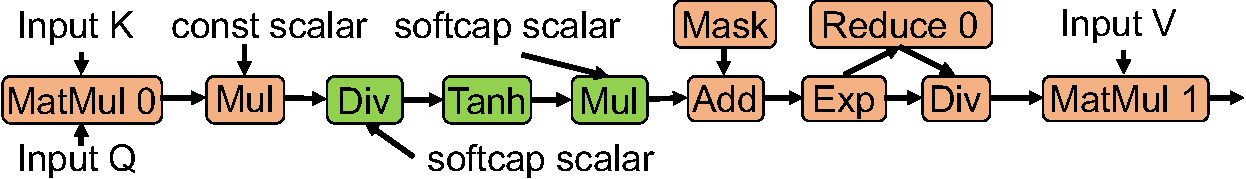
\includegraphics[width=0.75\linewidth]{figures/flashtensor/exp_gemma2-crop.pdf}
    \end{minipage}
    \vspace{-0.5em}
    \caption*{\small (a) 标准注意力与 Gemma2 的差异}
    
    \begin{minipage}[t]{\linewidth}
        \centering
        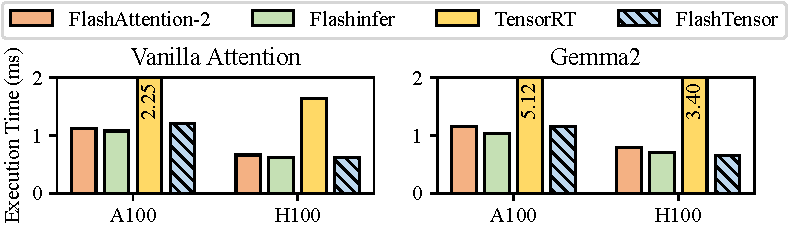
\includegraphics[width=0.7\linewidth]{figures/flashtensor/attn_time-crop.pdf}
    \end{minipage}
    \vspace{-0.5em}
    \caption*{\small (b) 标准注意力与 Gemma2 的执行时间}
    
    \caption{与算子库的对比}
    \label{fig:lib_cmp}
\end{figure}

\subsection{算子库对比实验}
本研究进一步将 FlashTensor 和 TensorRT 与手工调优的算子库 FlashAttention 和 FlashInfer 进行对比,这两个库均仅支持标准注意力(Vanilla Attention)和 Gemma2。  

% \begin{figure}[htbp]
%     \centering
%     % \vspace{-0.5em}
%     \begin{minipage}[ht]{\linewidth}
%         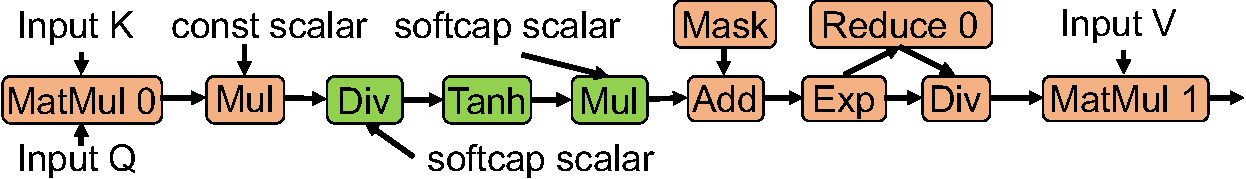
\includegraphics[width=\linewidth]{figures/flashtensor/exp_gemma2-crop.pdf}
%     \end{minipage}
%     % \vspace{-1em}
%     \\
% \centering \small (a) 标准注意力与 Gemma2 的差异。绿色算子为 Gemma2 的额外结构。  
%     \begin{minipage}[ht]{\linewidth}
%         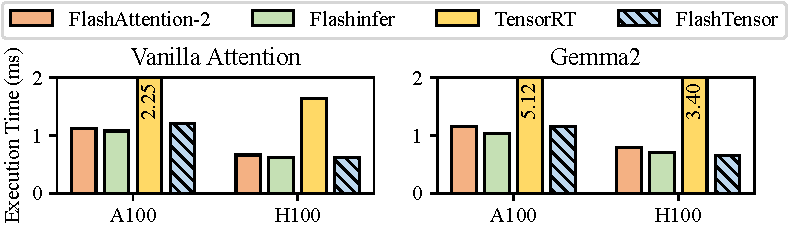
\includegraphics[width=\linewidth]{figures/flashtensor/attn_time-crop.pdf}
%     \end{minipage}
%     % \vspace{-1em}
%     \\
% \centering \small (b) 标准注意力与 Gemma2 的执行时间。截断条形图上标注了执行时间(ms)。  
%     % \vspace{-0.7em}
%     \caption{与算子库的对比}
%     % \vspace{-1.5em}
%     \label{fig:lib_cmp}
% \end{figure}  



如\Cref{fig:lib_cmp}(a) 所示,Gemma2~\cite{team2024gemma2} 在标准注意力中引入了逻辑软上限。
在\Cref{fig:lib_cmp}(b) 中,FlashTensor 与 FlashInfer 和 FlashAttention 实现了相当的性能——后两者均采用基于领域知识和人工调优的手工算子,截断条形图上标注了执行时间(ms)。
尽管 FlashTensor 未超越这些算子库,但其优势在于无需手动调优即可跨多种场景实现泛化和优化。




\subsection{性能分解分析}
本研究进行了分解分析以展示FlashTensor各个组件的性能影响,如\Cref{fig:breakdown}所示。
\begin{figure}[ht]
    \centering
    % \vspace{-1.8em}
    % \vspace{-1.6em}
    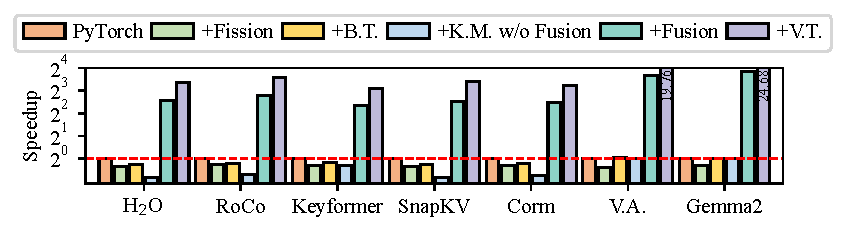
\includegraphics[width=0.85\linewidth]{figures/flashtensor/breakdown.pdf}
    % \vspace{-1.8em}
    \caption{H100上核心模块的性能分解分析}
    % \vspace{-0.5em}
    \label{fig:breakdown}
\end{figure}

基线为PyTorch,加速比为1。
FlashTensor首先应用算子裂变(Fission)将复杂算子分解为基本算子,例如将{Softmax}转换为{Exp}、{Reduce}和{Div}。
这会引入更小的算子,但增加内存访问量,从而降低整体性能。
接下来,提出基于广播属性的变换(B.T.)以最小化中间张量的大小。
这不仅提升了性能,还通过满足硬件约束为未来的融合操作创造了条件。
然后采用内核映射(K.M. w/o Fusion)来识别具有高并行效率的凸和非凸内核。
所识别的内核会重新计算一些算子以解决非凸内核的循环依赖问题,因此在未融合的情况下仍会导致性能下降。
融合操作通过减少内存访问开销并利用所识别内核的高并行效率,带来了最显著的性能提升,如\Cref{fig:breakdown}所示,加速比可达14.2倍。
最后,基于值属性的变换(V.T.)利用因果掩码消除冗余计算,在所有模型上进一步实现了近2倍的额外加速。



% \subsection{各阶段分析}
本研究进一步进行了各阶段分析,以分别展示变换和内核识别规则对性能的影响。

(1)\textbf{变换阶段}:
FlashTensor提出了一系列基于广播属性的变换规则,以最小化中间张量的大小。
如\Cref{tab:transform}所示,序列长度为4096时,中间张量的总大小显著减少了约3 GiB,这与\Cref{fig:seqlen_mem_flops}一致,实现了更低的内存使用和内存访问开销。此外,变换阶段的搜索成本非常小,约为数百毫秒。


\begin{table}[ht]
    \centering
    % \footnotesize
    \caption{基于广播变换的中间张量大小变化和执行时间}
    % \vspace{-0.5em}
    \begin{tabular}{ccc}
       \toprule
       模型  & 中间张量大小变化 & 时间(ms) \\
       \hline
       \(H_{2}O\)  & -3.30 GiB & 169.1 \\
       % \hline
       RoCo  & -3.18 GiB & 161.57 \\
       % \hline
       Keyformer  & -3.28 GiB & 223.69 \\
       % \hline
       SnapKV  & -3.30 GiB & 172.2 \\
       % \hline
       Corm  & -3.30 GiB & 166.5 \\
       % \hline
       标准注意力  & -3.98 GiB & 187.25 \\
       % \hline
       Gemma2  & -3.39 GiB & 238.25 \\
       \bottomrule
    \end{tabular}
    \label{tab:transform}
    % \vspace{-1.5em}
\end{table}




(2)\textbf{内核映射阶段}:
在确定最佳内核映射策略时,FlashTensor由于进一步引入了非凸内核定义,面临着巨大的搜索空间。
如\Cref{tab:search}所示,\#Op表示核心模块中的算子数量。\#Candidate表示剪枝后的候选数,括号内为可能的候选数。
即使算子数量较少,搜索空间仍然非常庞大。
例如,Keyformer的注意力模块仅包含24个算子,但整个搜索空间的大小达到了1.69亿。

如\Cref{tab:search}所示,Korch和TVM的调优时间很长,至少约2小时,但仍只能找到次优策略。
较长的调优时间主要来自对每个识别出的候选内核进行性能分析,需要大量时间来发现有效的调度方案。
然而,尽管FlashTensor的候选内核数量比Korch多得多,但本研究考虑了张量属性并有效剪枝了可能性能较差的候选内核,显著减少了候选集,从而能够在秒级快速选择最佳内核。

\begin{table}[ht]
    \centering
    % \footnotesize
    \caption{搜索性能}
    % \vspace{-0.5em}
    \begin{tabular}{cccccc}
    \toprule
      \multirow{2}{*}{模型} &  \multirow{2}{*}{\#Op}  & \#Candidate& \multicolumn{3}{c}{端到端搜索时间} \\
                              &  & (可能候选数)& FlashTensor & TVM & Korch \\
      \hline
      \(H_{2}O\)      & 16 & 5 (297K) & 3.03秒    & 1.8小时   & 1.6小时\\
      % \hline
      RoCo      & 19 & 7 (260万) & 8.40秒    & 2.3小时   & 3.5小时\\
      % \hline
      Keyformer & 24 & 10 (1.69亿) & 251.20秒 &3.3小时    & 失败 \\
      % \hline
      SnapKV    & 17 & 5 (20.7万) & 2.97秒    & 2.1小时   & 2.1小时\\
      % \hline
      Corm      & 17 & 5 (48万) & 4.14秒    & 失败 & 3.0小时\\
      % \hline
      V.A. & 15 & 4 (7万) & 2.42秒          & 1.5小时   & 1.4小时\\
      % \hline
      Gemma2    & 19  & 4 (170万) & 10.61秒  & 1.6小时   & 2.6小时 \\
      \bottomrule
    \end{tabular}
    \label{tab:search}
    % \vspace{-1.5em}
\end{table}


\section{结论}
本研究提出了 FlashTensor,这是一个利用细粒度张量属性优化张量程序的系统,旨在解决大模型后训练过程中,特别是长上下文任务中,因中间张量庞大而导致的内存开销大、算子计算效率低的问题。
本章首先总结了归约依赖、广播、大小和值这四个关键的张量属性,并设计了张量属性识别器,通过基于数据流的算法系统地分析计算图,准确捕获每个张量的属性。
然后,基于这些属性,本研究提出了张量属性感知优化方法,包括代数等价图变换和非凸内核映射,同时采用轻量级方案搜索方法,以找到最优的优化方案。
实验结果表明,与八种最先进的方法相比,FlashTensor 在 H100 上的端到端性能和核心模块性能平均加速比分别达到 1.50 倍和 3.24 倍,在 A100 上分别为 1.86 倍和 3.70 倍。

% 未来,本研究计划进一步扩展 FlashTensor 的应用范围,将其应用于更多类型的 DNN 模型和任务中。同时,我们将探索如何更好地结合硬件特性,进一步优化张量属性感知的优化策略,以实现更高的计算效率和更低的资源消耗。此外,我们还将研究如何将 FlashTensor 与其他深度学习优化技术相结合,形成更强大的优化框架,推动深度学习在更多领域的应用和发展。
 % FlashTensor
% !TeX root = ../thuthesis-example.tex

\chapter{基于弹性张量的大模型微调内存优化}

\section{概述}

大语言模型 [1, 30, 34, 39](LLMs)正日益普及。
与此同时,个性化以及支持个性化的微调技术 [7, 38, 40] 已成为大模型后训练领域的热门话题。
微调通常在有限的数据和典型的硬件配置下完成 [8, 10, 45],并且需要快速生成多个微调模型 [11, 16, 47]。
然而,由于大语言模型参数数量巨大,进行全参数微调难以满足上述要求 [15, 35, 46]。

为解决这一问题,研究人员提出了参数高效微调(Parameter-efficient finetuning, PEFT)。
与全参数微调不同,PEFT 从大模型的预训练权重出发,仅训练一小部分权重,同时冻结大部分权重 [14, 21, 26, 32, 42]。
这大幅减少了训练模型的计算量和存储需求(因为只需存储训练的那部分权重),同时仍能实现理想的模型性能。因此,PEFT 现已成为微调的主流方法 [6, 15, 23]。

在微调过程中,每个设备存储模型权重以及训练过程中生成的中间结果(激活值)。权重和激活值的大小与模型规模相关,大型模型的参数规模可达数十亿甚至数百亿。然而,单个 GPU 的内存限制通常仅为几十 GB。因此,权重和激活值需要在多个设备间进行划分,由此产生的通信开销成为性能瓶颈 [10, 45]。

内存可用于优化通信,这对训练性能至关重要。对于权重而言,更多的本地可用权重可以减少训练过程中的通信量;对于激活值,使用更大的批量大小虽然会增加激活值的内存需求,但可以降低每个样本的通信量。如图 1(a)所示,随着内存使用量的增加,不同模型的吞吐量能够得到显著提升。

现有的训练优化方法从内存角度展开。Deepspeed [33] 和 Torch-FSDP [43] 采用数据并行和零冗余优化(ZeRO)方法,为每个设备分配一部分样本。Megatron [20] 集成了数据并行、张量并行和流水线并行,对模型权重进行划分以减少通信开销。然而,由于以下两个原因,它们仍然无法充分利用内存:

激活值的峰谷模式:由于微调过程中反向传播的特性,在前向传播阶段首先生成的激活值直到反向传播的最后阶段才会被使用和释放。如图 1(c)所示,这种先进后出(FILO)的工作流程导致激活值内存使用呈现峰谷模式,造成大量内存未被充分利用(白色部分)。
静态划分的权重:激活值的内存使用在运行时动态变化,而权重在训练前被静态划分,并且在训练过程中不会进行调整。这种限制使得权重无法根据当前内存使用情况及其变化趋势进行动态调整。如图 1(c)所示,静态划分的权重无法利用激活值在低谷区域留下的内存空间。

因此,如图 1(b)所示,现有框架的时间平均内存利用率较低。其根本原因可归结为激活值和权重内存的静态调度:激活值以固定的速度和顺序产生和消耗,而静态分配的权重无法利用激活值留下的内存空间。

经观察,在 PEFT 中,权重和激活值的内存都可以进行动态高效的调整:对于 PEFT 中的权重,由于大部分权重被冻结,在不同设备上复制这些权重不会引入额外的同步开销。同时,通过细粒度地改变计算执行顺序,可以灵活修改驻留在内存中的激活值的大小和生命周期。

基于此观察,本章提出弹性张量的概念,以统一权重和激活值的动态内存管理。张量(权重和激活值)的大小在运行时动态调整,使权重内存和激活值内存之间的权衡适应当前内存使用情况和训练过程。在收集完整权重进行计算时调整权重内存;通过细粒度地生成、保存检查点和消耗激活值,灵活确定激活值的生命周期,从而调整其内存使用量。如图 1(d)所示,权重可以填充激活值内存的低谷区域,减少通信量;激活值可以降低峰值内存使用量,保持较高的内存利用率。

基于弹性张量,本章构建了 mTuner,这是一个具有高内存利用率的微调系统,可提高 PEFT 效率。mTuner 在运行时利用弹性权重和激活值,实现高内存利用率以节省通信量。在配备八个 GPU 的服务器上,对基于 Transformer、参数规模从 70 亿到 700 亿的大语言模型进行评估,结果表明,与 Deepspeed [33] 和 Megatron [20] 等最先进的训练系统相比,mTuner 可将微调性能提升最高达 1.51 倍(平均提升 1.28 倍)。mTuner 的吞吐量超过每秒 30,000 个标记,并且能够在 3 小时内使用 Llama-2 13B 模型对数学数据集 [12] 进行微调。

本文做出了以下贡献:

对 PEFT 的内存使用情况进行了详细分析,其主要包括权重和激活值;
提出弹性张量,能够灵活动态地调整权重和激活值的内存使用量;
基于弹性张量构建 mTuner,使执行计划能够适应内存状态,实现高效微调;
在参数规模从 70 亿到 700 亿的各种大语言模型上对 mTuner 进行评估,在 PCIe GPU 服务器上实现了最高 1.51 倍(平均 1.28 倍)的吞吐量提升,并且能够在 3 小时内微调模型以适应特定领域。

\section{mTuner系统概述}
图 3 展示了 mTuner 的系统概述。mTuner 的设计基于微调过程中张量的特殊属性--张量的弹性:权重和激活值张量的内存使用量都可以灵活动态地变化。第 4 节将分别深入探讨权重和激活值的张量弹性,讨论改变它们大小的方法以及相关的成本和收益。

接着介绍执行计划如何适应权重和激活值的弹性。因此XXXXXXXXXXXXXXXXXXXXXXXXXXX,mTuner 能够通过利用弹性张量实现自适应内存的训练计划。第 5 节将探讨 mTuner 如何感知内存状态。并根据内存状态,开发自适应内存的执行计划,利用张量弹性针对不同的内存状态进行优化,之后将介绍 mTuner 如何根据硬件设置和模型结构搜索具体的执行计划。


\section{弹性张量}
\label{mtuner:sec:elastic-tensor}

在微调过程中,需要长时间驻留在内存中的张量会占用大量内存,这包括分配给设备的权重内存以及设备计算过程中生成的中间结果(激活值)。本章研究发现,在 PEFT 的背景下,这些张量的内存大小可以进行调整。通过各种方式,可以增加或减少权重和激活值的内存使用量,同时需要考虑执行成本和收益之间的权衡。

\subsection{权重弹性}

\subsection{冻结权重}

由于 PEFT 区分基础模型和适配器的设计,其大部分权重(来自基础模型的权重)在训练过程中不会被更新,这些权重被称为冻结权重。尽管冻结权重不会更新,但它们仍然参与前向和后向计算(分别用于获取激活值和计算激活值的梯度)。因此,在传统的并行训练系统中,它们被视为普通权重。然而,我们发现由于这些冻结权重保持不变,它们可以在不同设备上冗余存储而不引入额外的同步开销。也就是说,对于在 D 个设备上进行的分布式微调,每个设备上权重的存储比例可以从\(\frac{1}{D}\)(全分片)连续变化到 100\%(全复制)。我们将这些存储比例可连续变化的权重称为弹性权重。

\subsubsection{权重大小的动态调整}

如图 4(a)和(b)所示,在执行一个算子时,每个设备通过通信(解分片,unshard)获取其完整权重,然后用于计算。计算完成后,收集到的权重被释放(重新分片,reshard)。
由于设备在计算过程中拥有完整的权重,mTuner 可以在不产生额外通信开销的情况下重新调整权重大小。在图 4(c)的示例中,在计算前,每个设备仅拥有算子权重的\(\frac{1}{D}\),计算后调整为\(\frac{2}{D}\)。这种动态调整可以在每次使用权重进行计算时进行,我们将这些时刻称为调整点。在一次迭代中,每个算子的权重至少有两个调整点:前向计算时和反向计算时。如果应用激活值检查点的重新计算,调整点可能会多于两个。mTuner 可以在这些调整点动态改变权重大小,以适应不同的内存使用情况。

\subsubsection{弹性权重的搜索空间}

弹性权重的大小可以在两个维度上进行调整:算子内和算子间。在算子内维度上,对于给定的算子,mTuner 可以将单个设备上存储的权重大小从\(\frac{1}{D}\)调整到 100\%。
然而,如果将弹性权重大小设置为\(\frac{k}{D}\),只有当 k 是 D 的因数时,才能缩小通信范围(从 D 个设备间的通信缩小到\(\frac{D}{k}\)个设备间的通信),从而显著提高通信效率。因此,在算子内维度上,mTuner 仅在 k 是 D 的因数时将弹性权重大小设置为\(\frac{k}{D}\)。例如,在使用八个 GPU 进行微调的情况下,每个算子的权重大小仅会选择 12.5\%、25\%、50\% 或 100\%。尽管算子内维度的这种选择策略可能会限制权重大小的灵活性,但在算子间维度上,不同的算子可以独立选择不同的弹性权重大小。由于大语言模型由大量算子组成,通过组合不同权重大小的算子,可以灵活配置整体弹性权重大小,使其连续覆盖从\(\frac{1}{D}\)到 100\% 的值。

\subsection{激活弹性}
在参数高效微调(PEFT)中,mTuner 还可以使激活具备弹性,以缓解因峰谷内存模式导致的内存利用率低下问题。我们发现,激活在内存中累积的主要原因是其先进后出(FILO)模式,以及由此产生的激活驻留时间长。因此,mTuner 采用两种方法来缩短生成的激活的生命周期,从而减少 FILO 模式带来的问题。第一种方法是提高反向计算的执行优先级,优先消耗前向传播过程中生成的激活;第二种方法是丢弃部分激活,并在反向传播过程中重新生成这些激活。
\subsubsection{提高反向计算优先级}
激活在前向传播阶段生成,在反向传播阶段使用并释放。因此,更早地执行反向计算可以缩短生成的激活的生命周期,使其更早地释放,减少在内存中的驻留时间。然而,在前向 - 反向计算范式中,必须先计算所有前向算子以获取损失,然后才能进行反向计算,这个顺序是不可改变的。为了便于更早地执行反向计算,我们提出沿样本维度拆分和重新排列计算顺序。
如图 5(a)所示,对于在四个输入样本上训练一个 4 层模型,典型的过程是将它们一起处理,先执行四个前向计算,然后执行四个反向计算。如图 5(b)所示,这个过程导致四个样本在前向传播结束时生成的激活都驻留在内存中,直到反向传播开始。由于所有激活都累积起来,内存使用量达到峰值。
为了更早地释放激活,mTuner 将样本划分为更小的批次,每个批次包含一个或多个样本。然后,对每个批次依次执行前向和反向计算,而不是将所有样本一起处理。如图 5(c)所示,对于四个样本的批次,mTuner 将它们分成两个批次,每个批次包含两个样本。它先对第一个批次执行前向计算,然后执行反向计算,释放第一个批次生成的激活。然后,对第二个批次重复相同的过程。通过这种方式,每个批次生成的激活在反向计算完成后立即释放,而不是累积到所有前向计算完成后,从而降低了峰值内存使用量。
\subsubsection{激活重计算}
除了重新排列计算顺序外,mTuner 还采用激活重计算技术进一步减少激活内存使用。激活重计算是一种通过重新计算激活而不是将其存储在内存中来减少激活内存占用的方法。在前向传播过程中,mTuner 不存储所有生成的激活,而是仅存储少量关键激活,这些关键激活足以在反向传播过程中重新计算其余激活。在反向传播过程中,mTuner 使用存储的关键激活重新计算所需的激活,而不是从内存中读取它们。
如图 6 所示,对于一个 4 层模型,mTuner 可以选择仅存储第 1 层和第 3 层的激活作为关键激活。在反向传播过程中,当需要第 2 层的激活时,mTuner 使用存储的第 1 层激活重新计算第 2 层的激活。通过这种方式,mTuner 可以显著减少激活内存使用,因为它只需要存储少量关键激活,而不是所有生成的激活。然而,激活重计算并非没有代价。由于在反向传播过程中需要重新计算激活,这会增加计算时间。因此,mTuner 需要在激活内存使用和计算时间之间进行权衡,以确定要存储的关键激活的最佳数量。
\subsubsection{激活弹性的搜索空间}
激活弹性的大小可以在两个维度上进行调整:样本维度和层维度。在样本维度上,mTuner 可以调整批次大小,即将样本划分为不同大小的批次。较小的批次大小可以更早地释放激活,降低峰值内存使用量,但会增加计算开销,因为每个批次都需要单独的前向和反向计算。较大的批次大小可以减少计算开销,但会增加峰值内存使用量。因此,mTuner 需要根据可用内存和计算资源在样本维度上选择合适的批次大小。
在层维度上,mTuner 可以选择存储哪些层的激活作为关键激活。不同的层选择会导致不同的激活内存使用和计算时间。存储更多层的激活作为关键激活可以减少反向传播过程中的计算时间,但会增加激活内存使用。存储较少层的激活作为关键激活可以减少激活内存使用,但会增加反向传播过程中的计算时间。因此,mTuner 需要在层维度上找到激活内存使用和计算时间之间的最佳平衡。
\section{自适应内存执行计划}
在\Cref{mtuner:sec:elastic-tensor}中,我们讨论了权重和激活的弹性,以及它们在内存使用方面的动态调整能力。在本节中,我们将介绍 mTuner 如何利用这些弹性张量来制定自适应内存执行计划,以适应不同的内存状态并优化微调性能。
\subsection{内存状态感知}
为了制定自适应内存执行计划,mTuner 首先需要感知内存状态。mTuner 通过监测设备内存使用情况和通信开销来获取内存状态信息。具体来说,mTuner 跟踪以下指标:
权重内存使用量:每个设备上存储的权重的大小。这包括分配给设备的固定权重和动态调整的弹性权重。
激活内存使用量:每个设备上存储的激活的大小。这包括当前驻留在内存中的激活和由于激活重计算而存储的关键激活。
空闲内存量:每个设备上当前未被使用的内存大小。空闲内存量是通过从设备的总内存容量中减去权重内存使用量和激活内存使用量得到的。
通信开销:在一次迭代中,设备之间为了获取完整权重和交换激活而进行通信所消耗的时间和带宽。通信开销是评估微调性能的重要指标,因为它直接影响训练速度。
mTuner 定期收集这些指标,并根据它们来评估当前的内存状态。例如,如果空闲内存量较低,mTuner 会认为内存处于紧张状态,需要采取措施减少内存使用。如果通信开销较高,mTuner 会尝试调整权重和激活的分布,以减少通信量。
\subsection{执行计划制定}
根据感知到的内存状态,mTuner 制定自适应内存执行计划。执行计划包括如何在设备之间分配权重、如何生成和管理激活,以及何时进行计算等决策。
当内存处于紧张状态时,mTuner 会优先减少内存使用。对于权重,它会减少每个设备上存储的弹性权重大小,以释放更多内存用于激活。例如,如果当前空闲内存量不足以存储所有激活,mTuner 可能会将某些算子的弹性权重大小从 100\% 调整为 50\%,从而为激活腾出空间。对于激活,mTuner 会采用较小的批次大小和更多的激活重计算,以降低峰值内存使用量。较小的批次大小可以更早地释放激活,而更多的激活重计算可以减少存储的激活数量。
当内存相对充裕时,mTuner 会尝试提高计算效率。对于权重,它会增加每个设备上存储的弹性权重大小,以减少通信量。例如,如果空闲内存量较多,mTuner 可能会将更多算子的弹性权重大小设置为 100\%,这样每个设备在计算时就不需要与其他设备进行通信来获取完整权重。对于激活,mTuner 会采用较大的批次大小和较少的激活重计算,以减少计算开销。较大的批次大小可以减少前向和反向计算的次数,而较少的激活重计算可以减少重新计算激活的时间。
\subsection{执行计划搜索}
mTuner 使用搜索算法来找到最佳的执行计划。由于权重和激活弹性的搜索空间较大,穷举搜索所有可能的执行计划是不现实的。因此,mTuner 采用启发式搜索算法来有效地探索搜索空间。
mTuner 从一个初始执行计划开始,该计划可以是默认的静态执行计划或基于一些简单规则生成的计划。然后,mTuner 通过对当前执行计划进行小的调整来生成候选执行计划。这些调整可以包括改变某个算子的弹性权重大小、调整批次大小或选择不同的激活重计算层。对于每个候选执行计划,mTuner 评估其性能,包括内存使用量、通信开销和训练吞吐量。根据评估结果,mTuner 选择性能最佳的候选执行计划作为新的当前执行计划,并继续生成新的候选执行计划进行评估。这个过程会持续进行,直到达到预定的搜索预算(例如,一定数量的迭代次数或时间限制)或找到满意的执行计划。
mTuner 还利用硬件设置和模型结构的信息来指导搜索过程。例如,如果设备具有高带宽通信网络,mTuner 可能会更倾向于选择那些虽然通信量较大但计算效率更高的执行计划。如果模型具有较多的层或较大的参数规模,mTuner 会更加关注激活内存使用和权重分配,以避免内存不足和通信瓶颈。


\section{实验评估}
\subsection{实验设置}
本章在配备八个 NVIDIA A100 GPU 的服务器上进行实验,每个 GPU 具有 80GB 内存。本章评估了 mTuner 在不同规模的基于 Transformer 的大语言模型上的性能,包括 7B、13B、30B 和 70B 参数模型。本章使用 PyTorch 作为深度学习框架,并将 mTuner 与两个最先进的训练系统进行比较:Deepspeed [33] 和 Megatron [20]。
本章使用 Llama-2 [30] 作为基础模型,并在各种数据集上进行微调,包括用于通用语言任务的 C4 [37] 和用于特定领域任务的数学数据集 [12]。本章使用 AdamW 优化器 [27] 进行训练,学习率设置为1e-4,批量大小根据模型规模和可用内存进行调整。
\subsection{性能比较}
图 7 展示了 mTuner 与 Deepspeed 和 Megatron 在不同模型规模上的吞吐量比较。结果表明,mTuner 在所有模型规模上都显著优于 Deepspeed 和 Megatron。在 7B 模型上,mTuner 的吞吐量比 Deepspeed 高 1.23 倍,比 Megatron 高 1.18 倍。在 13B 模型上,mTuner 的吞吐量比 Deepspeed 高 1.35 倍,比 Megatron 高 1.27 倍。在 30B 模型上,mTuner 的吞吐量比 Deepspeed 高 1.42 倍,比 Megatron 高 1.34 倍。在 70B 模型上,mTuner 的吞吐量比 Deepspeed 高 1.51 倍,比 Megatron 高 1.45 倍。平均而言,mTuner 的吞吐量比 Deepspeed 高 1.28 倍,比 Megatron 高 1.22 倍。
这些结果表明,mTuner 能够有效地利用弹性张量来优化内存使用和减少通信开销,从而显著提高微调性能。通过动态调整权重和激活的内存使用量,mTuner 能够更好地适应不同模型规模和内存状态,实现更高的训练效率。
\subsection{内存使用分析}
图 8 展示了 mTuner 与 Deepspeed 和 Megatron 在 13B 模型上的内存使用情况比较。结果表明,mTuner 能够更有效地利用内存。在峰值内存使用方面,mTuner 比 Deepspeed 低 23\%,比 Megatron 低 18\%。这是因为 mTuner 通过调整批次大小和采用激活重计算技术,降低了激活的峰值内存使用量。在平均内存使用方面,mTuner 比 Deepspeed 高 12\%,比 Megatron 高 8\%。这是因为 mTuner 在内存相对充裕时,通过增加弹性权重大小来减少通信量,从而提高了内存利用率。
这些结果表明,mTuner 在内存管理方面具有优势。通过灵活调整权重和激活的内存使用量,mTuner 能够在保证不超过设备内存限制的前提下,充分利用空闲内存,提高内存利用率,同时降低峰值内存使用量,避免内存不足的问题。
\subsection{特定领域微调}
本章还评估了 mTuner 在特定领域微调任务中的性能。本章使用 Llama-2 13B 模型在数学数据集 [12] 上进行微调,以增强其数学能力。图 9 展示了 mTuner 与 Deepspeed 和 Megatron 在数学数据集上的微调时间比较。结果表明,mTuner 能够显著缩短微调时间。mTuner 在 3 小时内完成了微调,而 Deepspeed 需要 4.5 小时,Megatron 需要 5 小时。
这些结果表明,mTuner 不仅在通用语言任务的微调中表现出色,而且在特定领域任务的微调中也具有显著优势。通过提高微调性能,mTuner 能够更快地使模型适应特定领域,提高模型在特定领域任务中的表现。
\section{结论}
本章提出了 mTuner,这是一个利用弹性张量在多 GPU 服务器上加速参数高效微调的系统。通过对 PEFT 中内存使用情况的详细分析,发现权重和激活的内存都可以进行动态高效的调整。基于此,提出了弹性张量的概念,使张量的大小能够在运行时动态灵活地改变,从而提高内存利用率。
基于弹性张量构建了 mTuner,它能够感知内存状态并制定自适应内存执行计划。实验结果表明,与最先进的训练系统相比,mTuner 在各种规模的大语言模型上实现了显著的性能提升,吞吐量最高提升可达 1.51 倍(平均提升 1.28 倍)。mTuner 还能够在 3 小时内对 Llama - 2 13B 模型进行微调,以增强其数学能力。
未来,计划进一步探索如何将 mTuner 应用于更广泛的模型和任务,并研究如何在不同的硬件平台上优化 mTuner 的性能,还将研究如何将 mTuner 与其他先进的训练技术相结合,以进一步提高微调效率。

% \section{论文的语言及表述}

% 除国际研究生外,学位论文一律须用汉语书写。
% 学位论文应当用规范汉字进行撰写,除古汉语研究中涉及的古文字和参考文献中引用的外文文献之外,均采用简体汉字撰写。

% 国际研究生一般应以中文或英文书写学位论文,格式要求同上。
% 论文须用中文封面。

% 研究生学位论文是学术作品,因此其表述要严谨简明,重点突出,专业常识应简写或不写,做到立论正确、数据可靠、说明透彻、推理严谨、文字凝练、层次分明,避免使用文学性质的或带感情色彩的非学术性语言。

% 论文中如出现一个非通用性的新名词、新术语或新概念,需随即解释清楚。



% \section{论文题目的写法}

% 论文题目应简明扼要地反映论文工作的主要内容,力求精炼、准确,切忌笼统。
% 论文题目是对研究对象的准确、具体描述,一般要在一定程度上体现研究结论,因此,论文题目不仅应告诉读者这本论文研究了什么问题,更要告诉读者这个研究得出的结论。
% 例如:“在事实与虚构之间:梅乐、卡彭特、沃尔夫的新闻观”就比“三个美国作家的新闻观研究”更专业、更准确。



% \section{摘要的写法}

% 论文摘要是对论文研究内容的高度概括,应具有独立性和自含性,即应是 一篇简短但意义完整的文章。
% 通过阅读论文摘要,读者应该能够对论文的研究 方法及结论有一个整体性的了解,因此摘要的写法应力求精确简明。
% 论文摘要 应包括对问题及研究目的的描述、对使用的方法和研究过程进行的简要介绍、 对研究结论的高度凝练等,重点是结果和结论。

% 论文摘要切忌写成全文的提纲,尤其要避免“第 1 章……;第 2 章……;……”这样的陈述方式。



% \section{引言的写法}

% 一篇学位论文的引言大致包含如下几个部分:
% 1、问题的提出;
% 2、选题背 景及意义;
% 3、文献综述;
% 4、研究方法;
% 5、论文结构安排。
% \begin{itemize}
%   \item 问题的提出:要清晰地阐述所要研究的问题“是什么”。
%     \footnote{选题时切记要有“问题意识”,不要选不是问题的问题来研究。}
%   \item 选题背景及意义:论述清楚为什么选择这个题目来研究,即阐述该研究对学科发展的贡献、对国计民生的理论与现实意义等。
%   \item 文献综述:对本研究主题范围内的文献进行详尽的综合述评,“述”的同时一定要有“评”,指出现有研究状态,仍存在哪些尚待解决的问题,讲出自己的研究有哪些探索性内容。
%   \item 研究方法:讲清论文所使用的学术研究方法。
%   \item 论文结构安排:介绍本论文的写作结构安排。
% \end{itemize}



% \section{正文的写法}

% 本部分是论文作者的研究内容,不能将他人研究成果不加区分地掺和进来。
% 已经在引言的文献综述部分讲过的内容,这里不需要再重复。
% 各章之间要存在有机联系,符合逻辑顺序。



% \section{结论的写法}

% 结论是对论文主要研究结果、论点的提炼与概括,应精炼、准确、完整,使读者看后能全面了解论文的意义、目的和工作内容。
% 结论是最终的、总体的结论,不是正文各章小结的简单重复。
% 结论应包括论文的核心观点,主要阐述作者的创造性工作及所取得的研究成果在本领域中的地位、作用和意义,交代研究工作的局限,提出未来工作的意见或建议。
% 同时,要严格区分自己取得的成果与指导教师及他人的学术成果。

% 在评价自己的研究工作成果时,要实事求是,除非有足够的证据表明自己的研究是“首次”、“领先”、“填补空白”的,否则应避免使用这些或类似词语。
  % MTuner
% !TeX root = ../thuthesis-example.tex

\chapter{基于轻量级上下文切换的后训练通信优化}


大语言模型(LLMs)的对齐近来备受关注,这凸显了确保这些先进人工智能系统以符合伦理规范且有益社会的方式运行的必要性。值得注意的是,InstructGPT [21]、ChatGPT [19] 系列模型(包括 OpenAI 的 GPT-4 [20]、谷歌的 Bard [6] 以及 Meta 的 LLaMA 2-Chat [26])的最新发展,都强调了对齐在这些模型中的重要性。实现这种对齐的主要方法是基于人类反馈的强化学习(RLHF),其中近端策略优化(PPO)是广泛认可的标准算法,它显著提升了大语言模型在包括自然语言处理 [9,19]、文本生成图像 [11,28] 等诸多深度学习任务中的可靠性。 
大语言模型对齐的范式与现有深度学习系统所针对的标准全参数微调或预训练方法存在显著差异。如图 1 所示,我们以大语言模型对齐中公认的标准算法 PPO 为例,来说明推理、典型微调(或预训练)和对齐这几种范式之间的区别。在微调过程中(如图 1(b)所示),仅需单个模型;而在对齐过程中(如图 1(c)所示),则需要多个模型,包括 Actor、Critic、Reference 和 Reward 模型。根据模型的工作负载特征(推理或微调)以及它们之间的数据依赖关系,该范式可分为多个阶段,且不同模型之间的数据依赖仅存在于阶段之间。此外,在后续讨论中,我们将模型的工作负载和模型本身统称为上下文。 
我们观察到,当前大语言模型对齐的标准方法具有以下不同特点: 

1.	异构模型和工作负载:PPO 等对齐方法涉及多种模型的协同参与,从而导致异构性。这种异构性源于两个方面:模型结构和工作负载。首先,不同模型的参数数量和结构存在显著差异;其次,对齐过程还引入了多样化的工作负载,如解码、推理和训练。因此,这些异构上下文使得对齐过程比标准微调更为复杂。 

2.	频繁的上下文切换:整个对齐过程涉及以循环方式执行不同模型的不同工作负载(上下文),从而导致频繁的上下文切换。上下文切换不仅发生在阶段之间,也发生在阶段内部,例如当一个阶段内的多个模型按顺序执行时。如此频繁的切换会引入大量开销,包括模型重新加载、参数更新、数据传输等。例如,DeepSpeed-Chat 在收集更新后的参数时会产生 12.43% 的开销。 
目前,已有大量深度学习系统被提出以应对不同的复杂场景,如推理和训练。然而,这些系统存在以下两个局限性: 

3.	仅专注于单个模型:现有研究 [10, 17, 18, 35] 专注于为单个模型优化算子、计算图和并行执行计划,但忽略了涉及多个模型协同训练的场景,错失了进行细粒度跨模型优化的机会。 

4.	忽视模型中的多样化工作负载:现有的推理 [10,13,32] 和训练系统 [29,30] 为其模型维持固定的工作负载,在执行过程中不需要更改配置(如并行执行计划)。在这些系统中,没有充分考虑对齐过程中所需的频繁上下文切换,从而导致了巨大且难以接受的成本。 

因此,我们认为在大语言模型对齐中,异构上下文之间的高效切换是一项关键挑战,并且这仍是一个有待解决的研究问题。 
为应对这些挑战,我们提出了 PUZZLE,这是一个将模型上下文视为核心要素的高效大语言模型对齐系统。我们研究了大语言模型对齐过程中的模型编排,充分考虑了其中涉及的异构上下文,并利用异构上下文之间的相似性来实现轻量级、流畅的上下文切换。具体而言,为了有效处理对齐过程中的异构上下文特性,PUZZLE 采用二维方法,同时考虑阶段内和阶段间的上下文切换。在每个阶段内,我们通过探索不同上下文之间的亲和力,并利用分时策略实现计算重叠,从而将切换成本降至最低。此外,为了减少阶段之间的切换开销,我们制定了基于相似性的方案,以找到通信成本最小的最优阶段间上下文切换方案。我们在配备多达 32 个 GPU 的不同集群上对 PUZZLE 进行了评估,结果表明,与最先进的 RLHF 训练系统 DeepSpeed-Chat [31] 相比,PUZZLE 在端到端训练中的加速比最高可达 2.12 倍。 
总之,我们做出了以下贡献: 

1.	我们从对齐问题中抽象出上下文的关键概念,并通过关注上下文切换确定了性能优化的方向。 

2.	我们提出了一种分时策略,用于探索阶段内不同上下文之间的亲和力,并将其整合到混合方案中。 

3.	我们制定了基于相似性的方案,以找到通信成本最小的最优阶段间上下文切换方案。 

4.	我们构建了 PUZZLE,将上述技术实现为一个端到端的训练系统,与现有最先进的系统相比,实现了高达 2.12 倍的加速。 


\section{挑战与动机}
如前所述,在大语言模型对齐过程中,异构上下文之间的高效切换(包括阶段内上下文切换和阶段间上下文切换)是一项关键挑战。在本节中,我们阐述实现高效阶段内和阶段间切换的动机。 
12.	阶段内上下文切换:大语言模型对齐过程中的多个模型和工作负载涉及异构上下文,并且由于一个阶段内的这些异构上下文之间不存在数据依赖关系,因此可以采用 2.1 节中介绍的多模型并行执行方案进行执行。我们观察到,所选方案在并行执行过程中常常出现大量空闲时间(如图 2 所示),这主要归因于以下原因:异构上下文之间存在显著差异,即便采用最优的方案组合,仍会产生空闲时间。如图 2(d)所示,我们的动机在于通过细粒度调度探索上下文之间的亲和力,目标是在相对最优的方案中实施分时策略,以最大限度地减少空闲时间。 
13.	阶段间上下文切换:在对齐过程中,同一模型的上下文可能具有不同的工作负载,例如生成(解码)和训练阶段。工作负载特征的差异导致最优并行执行方案完全不同。例如,图 3(a)展示了 LLaMA-7B 模型在不同并行执行方案下生成和训练的性能表现。为清晰起见,我们省略了数据并行维度(图中的数据并行维度固定为 1),其中(P, T)分别表示流水线并行和张量并行维度。此外,为了在不同阶段实现同一模型的最佳性能,还需要仔细考虑不同方案之间的参数重组开销,这是阶段间上下文切换成本的主要来源。如图 3(b)所示,该图展示了不同方案下的切换成本,我们观察到,对于相似性较高的方案,它们之间的切换成本要低得多。 


\section{概述}
我们提出了 PUZZLE,这是一个用于大语言模型的高效对齐系统,其名称源于每个异构上下文都类似于拼图的一块,我们的目标是将这些 “拼图块” 合理布局,并在系统中高效执行。 
图 4 展示了 PUZZLE 的系统概览。该系统的核心概念基于对齐过程中遇到的独特异构模型和工作负载属性(本文中称为上下文)。由于异构上下文特性,需要在阶段内和阶段间频繁切换,这会导致开销增加。PUZZLE 旨在通过挖掘阶段内和阶段间过程中的潜在机会,降低此开销并提升系统效率。 
在第 4 节中,我们通过探索不同上下文之间的亲和力,并利用分时策略实现计算重叠,从而最小化阶段内切换成本;在第 5 节中,我们介绍阶段间上下文切换,通过找到具有高度相似性且通信成本最小的最优并行执行方案,来降低阶段间切换成本。 
\section{基于亲和力的阶段内切换}
尽管现有的并行执行技术效率较高,但在大语言模型对齐方面仍有提升空间,尤其是在并行执行方案中的上下文切换过程中存在空闲时间。对齐过程中的异构上下文可划分为不同阶段,我们发现,对每个阶段内的上下文进行编排能够显著提升阶段内上下文切换效率。 
本节介绍基于亲和力的阶段内切换技术,该技术应用于 PUZZLE,用于探索不同上下文之间的布局和执行方案。首先,我们分析阶段内上下文切换的开销和潜在机会(4.1),并引入新的分时切换方案(4.2)以促进上下文协作;最后,将所有现有方法相结合,形成多样化的布局和执行策略空间,即混合方案(4.3)。 
\subsection{布局和执行方案的机会}
尽管此前已有研究探索了对模型布局和执行的支持,但一个普遍的局限在于缺乏对上下文之间协作的关注,在对齐过程的同一阶段内,计算效率仍有很大的提升空间。我们首先分析阶段内上下文切换的开销和潜在机会。 
14.	开销的定义:首先,我们分析阶段内上下文切换可能引入的开销类型。对于不共享资源的布局和执行方案,它们之间无需进行上下文切换,因此不会引入开销;然而,在资源共享的场景中,上下文按顺序执行,从而会引入开销。 
15.	潜在机会:如图 2(d)所示,我们观察到两个上下文可以实现重叠。这是因为 PUZZLE 采用了混合并行化,包括张量并行、数据并行和流水线并行。我们主要关注流水线并行带来的开销,通常称为 “流水线气泡”。这种开销会导致在流水线填满之前或接近完成时,某些设备处于空闲状态,进而影响整体吞吐量。此类 “流水线气泡” 可能导致不必要的计算,尤其是在存在依赖关系的场景中。 
16.	基于亲和力的方法:在涉及众多模型参与的对齐过程中,每个模型的并行策略可能存在显著差异。然而,根据为每个模型选择的并行策略,我们可以探索它们之间的亲和力。在此,亲和力是指当两种并行策略高度相似时,计算过程能够有效重叠。 
\subsection{分时切换方案}
本节介绍一种新的主要执行方案,该方案旨在降低阶段内上下文切换的开销,实现共享相同资源的不同上下文之间的细粒度分时。PUZZLE 在对齐过程中采用这种分时技术来探索上下文协作。 
我们首先回顾训练两个模型 A 和 B 的传统策略,其执行顺序为顺序执行。如图 5(a)所示,该示例展示了两个模型的训练过程,每个模型被划分为四个部分,每个部分分配给一个设备,形成四层流水线,工作流程还包括四个微批次,两个模型按顺序执行。然而,如图 5(a)中的灰色框所示,在两次上下文切换之间会产生大量 “气泡”,在这些空闲时间段内,设备处于闲置状态。因此,这种场景存在显著的优化空间,尤其是对于无依赖关系的任务执行。 
图 5(b)展示了分时技术的一个示例。通过将后续训练任务与前一个任务相结合,可以有效利用前一个任务的空闲时间。这种分时技术类似于操作系统中的进程并发,由于这些任务之间不存在依赖关系,因此可以并发执行。例如,在模型 B 的第一个微批次前向传播在模型 A 的第一个微批次反向传播之后立即执行,此时执行时间为 9,而不是延迟到 15。此外,图中所示的调度类似于在单个模型中完成八个微批次的训练。 
17.	理论加速比:在图 5(b)中,模型 2 的第一个微批次前向传播在模型 1 的第一个微批次反向传播之后开始,此时模型 1 处于冷却阶段,模型 2 处于预热阶段。设\(T^{f}\)表示每个前向传播的时间,\(T^{b}\)表示每个反向传播的时间,\(T^{idle}\)表示空闲时间。在顺序执行中,总时间 \(T_{seq} = 4(T^{f} + T^{b}) + T^{idle}\);而在分时执行中,总时间 \(T_{ts} = 4(T^{f} + T^{b}) - T^{idle}\)。因此,理论加速比 \(S = \frac{T_{seq}}{T_{ts}}=\frac{4(T^{f} + T^{b}) + T^{idle}}{4(T^{f} + T^{b}) - T^{idle}}\)。可以看出,空闲时间 \(T^{idle}\) 越大,加速比 \(S\) 越高。
实现:为了实现分时切换方案,我们需要解决两个关键问题:何时进行上下文切换以及如何进行上下文切换。
何时切换:在流水线并行中,每个设备负责模型的一个阶段,并且在每个微批次中,设备需要等待上一个阶段的设备完成计算并将数据传输过来后才能开始计算。因此,我们可以利用设备等待数据的时间来执行其他上下文的计算。具体来说,当一个设备完成了当前上下文的前向传播并且正在等待上一个阶段的设备传输反向传播的数据时,我们可以在这个设备上启动另一个上下文的前向传播。这样,两个上下文的计算就可以在时间上重叠,从而提高计算资源的利用率。
如何切换:在进行上下文切换时,我们需要确保两个上下文之间的数据不会相互干扰。为此,我们为每个上下文分配独立的内存空间,并且在切换上下文时,保存当前上下文的计算状态(如中间变量、梯度等),并加载下一个上下文的计算状态。这样,每个上下文的计算都可以独立进行,不会受到其他上下文的影响。
\subsection{混合方案}
虽然分时切换方案能够有效利用空闲时间,提高计算资源的利用率,但它并不能完全消除上下文切换的开销。此外,不同的上下文可能具有不同的计算特性和资源需求,单一的分时切换方案可能无法适用于所有情况。因此,我们提出了一种混合方案,将分时切换方案与其他现有的布局和执行方案相结合,以提供更灵活和高效的上下文管理方式。
具体来说,混合方案包括以下几个步骤:
方案选择:根据每个上下文的计算特性(如计算密集型或通信密集型)和资源需求(如内存需求、计算能力需求等),选择合适的布局和执行方案。例如,对于计算密集型的上下文,我们可以选择张量并行方案,以充分利用设备的计算能力;对于通信密集型的上下文,我们可以选择数据并行方案,以减少通信开销。
分时调度:对于选择了相同资源的上下文,我们采用分时切换方案进行调度,以实现计算重叠,减少空闲时间。在分时调度过程中,我们根据上下文之间的亲和力,确定它们的执行顺序和时间分配,以最大化计算资源的利用率。
动态调整:在执行过程中,我们实时监测系统的资源使用情况和上下文的执行状态,并根据监测结果动态调整布局和执行方案。例如,如果某个上下文的执行速度较慢,导致其他上下文等待时间过长,我们可以调整该上下文的并行策略或重新分配资源,以提高其执行速度。
通过混合方案,我们可以根据不同上下文的特点和系统的运行状态,灵活地选择和调整布局和执行方案,从而有效地降低阶段内上下文切换的开销,提高大语言模型对齐的效率。
\section{基于相似性的阶段间切换}
在大语言模型对齐过程中,阶段间上下文切换同样会带来显著的开销,主要源于不同阶段中同一模型的工作负载差异导致的最优并行执行方案不同,以及方案切换时的参数重组。为降低这些开销,我们提出基于相似性的阶段间切换策略,旨在找到通信成本最小的最优并行执行方案。
\subsection{并行执行方案的相似性度量}
为找到最优的阶段间切换方案,首先需要定义一种度量方式来评估不同并行执行方案之间的相似性。我们从两个维度来考虑方案的相似性:参数布局相似性和通信模式相似性。
参数布局相似性:大语言模型的参数在不同并行执行方案下的布局方式对切换成本有重要影响。我们通过比较不同方案中参数在设备间的分布情况来衡量参数布局相似性。具体而言,对于每个模型的参数,我们计算在两种方案下参数在相同设备上的比例。假设模型有 \(N\) 个参数,在方案 \(A\) 和方案 \(B\) 下,有 \(n\) 个参数位于相同的设备上,则参数布局相似性得分 \(S_{p} = \frac{n}{N}
\)。得分越高,表明两种方案的参数布局越相似,在切换时需要进行的参数重组操作就越少,从而降低切换成本。
通信模式相似性:不同的并行执行方案会导致不同的通信模式,包括通信的设备对、通信的数据量和通信的频率等。我们通过分析通信模式的这些要素来评估通信模式相似性。具体方法是,构建每个方案的通信矩阵,矩阵中的元素表示设备之间的通信关系和数据量。然后,计算两个通信矩阵之间的相似度。例如,可以使用余弦相似度来衡量两个通信矩阵的相似程度,设两个通信矩阵为 \(C_{A}\) 和 \(C_{B}\),则通信模式相似性得分 \(S_{c} = \frac{C_{A} \cdot C_{B}}{\vert\vert C_{A}\vert\vert \vert\vert C_{B}\vert\vert}\)。得分越高,说明两种方案的通信模式越相似,在切换时可以减少通信协议的重新配置和数据传输的调整,进而降低通信开销。
综合参数布局相似性和通信模式相似性,我们得到并行执行方案的总体相似性得分 \(S = \alpha S_{p} + (1 - \alpha) S_{c}\),其中 \(\alpha\) 是一个权重系数,用于平衡参数布局相似性和通信模式相似性的重要程度。通过实验,我们可以确定最优的 \(\alpha\) 值,以使得总体相似性得分能够最准确地反映方案切换成本。
\subsection{最优方案搜索}
在定义了相似性度量后,我们需要在所有可能的并行执行方案中搜索最优方案,以实现最小的阶段间上下文切换成本。由于可能的方案数量较多,穷举搜索是不可行的,因此我们采用启发式搜索算法。
我们从当前阶段的并行执行方案出发,通过对方案进行小的调整来生成候选方案。例如,可以改变流水线并行的阶段划分、调整张量并行的维度或者修改数据并行的分组方式等。对于每个候选方案,我们计算其与下一阶段目标方案的相似性得分,并评估切换到该候选方案所需的成本,包括参数重组成本和通信成本。成本评估可以通过模拟方案切换过程,计算参数传输量、设备间通信次数和时间等指标来实现。
然后,我们选择相似性得分最高且切换成本最低的候选方案作为下一阶段的执行方案。为了避免陷入局部最优解,我们还引入了随机搜索和模拟退火等策略,在一定程度上探索更广泛的方案空间。通过不断迭代搜索过程,我们能够找到接近最优的阶段间上下文切换方案,从而有效降低阶段间切换开销,提高大语言模型对齐的整体效率。
\section{实验评估}
\subsection{实验设置}
我们在多个配备不同数量 NVIDIA A100 GPU 的集群上对 PUZZLE 进行评估,集群的 GPU 数量从 8 个到 32 个不等,每个 GPU 具有 80GB 内存。实验中,我们以 LLaMA-7B、LLaMA-13B 和 LLaMA-30B 等基于 Transformer 架构的大语言模型为对象,使用 PyTorch 作为深度学习框架,并将 PUZZLE 与最先进的基于人类反馈的强化学习训练系统 DeepSpeed-Chat 进行对比。
在数据集方面,我们采用了多个公开的大规模数据集,包括用于生成训练数据的 CommonCrawl 语料库,以及用于构建奖励模型的人工标注数据集。训练过程中,我们使用近端策略优化(PPO)算法进行大语言模型对齐,并根据模型规模和数据集特点,合理调整超参数,如学习率设置在 \(1e^{-5}\) 到 \(5e^{-5}\) 之间,批次大小根据 GPU 内存和模型复杂度进行动态调整。
\subsection{性能对比}
图 6 展示了 PUZZLE 与 DeepSpeed-Chat 在不同模型规模和 GPU 数量下的端到端训练时间对比。结果表明,PUZZLE 在所有测试场景下均显著优于 DeepSpeed-Chat。当使用 8 个 GPU 对 LLaMA-7B 模型进行对齐训练时,PUZZLE 的训练时间比 DeepSpeed-Chat 缩短了 42\%;随着 GPU 数量增加到 32 个,在对 LLaMA-30B 模型进行训练时,PUZZLE 的加速比最高可达 2.12 倍。平均而言,与 DeepSpeed-Chat 相比,PUZZLE 在不同模型和 GPU 配置下的训练时间平均减少了 58\%,这充分证明了 PUZZLE 在提高大语言模型对齐效率方面的有效性。
\subsection{开销分析}
我们进一步分析了 PUZZLE 在阶段内和阶段间上下文切换过程中的开销,并与 DeepSpeed-Chat 进行对比。图 7(a)展示了阶段内上下文切换的空闲时间占比情况。可以看到,DeepSpeed-Chat 由于采用传统的顺序执行或简单的并行方案,阶段内存在大量空闲时间,平均空闲时间占比达到 35\%;而 PUZZLE 通过基于亲和力的分时切换方案和混合方案,有效减少了空闲时间,平均空闲时间占比仅为 12\%,显著提高了计算资源的利用率。
在阶段间上下文切换方面,图 7(b)显示了不同方案切换时的通信成本和参数重组成本。DeepSpeed-Chat 在切换并行执行方案时,由于没有考虑方案之间的相似性,导致通信成本和参数重组成本较高;相比之下,PUZZLE 采用基于相似性的阶段间切换策略,能够选择相似性高的方案进行切换,使得通信成本降低了 60\%,参数重组成本降低了 55\%。这些结果表明,PUZZLE 通过优化阶段内和阶段间的上下文切换,有效降低了整体开销,从而实现了更高的训练效率。
\subsection{扩展性评估}
为了评估 PUZZLE 的扩展性,我们测试了其在不同规模集群和模型上的性能表现。图 8 展示了随着 GPU 数量增加,PUZZLE 和 DeepSpeed-Chat 的训练吞吐量变化情况。结果显示,PUZZLE 在不同规模的集群上都能保持良好的扩展性,随着 GPU 数量从 8 个增加到 32 个,其训练吞吐量线性增长,增长幅度达到 2.8 倍;而 DeepSpeed-Chat 在 GPU 数量较多时,由于上下文切换开销的增加,扩展性受到限制,吞吐量增长幅度仅为 1.5 倍。这表明 PUZZLE 能够更好地适应大规模集群环境,在处理大规模大语言模型对齐任务时具有显著优势。
\section{相关工作}
\subsection{大语言模型训练优化}
近年来,众多研究致力于大语言模型的训练优化。一些工作聚焦于改进并行计算策略,例如 Megatron-LM [18] 通过混合并行化方法,结合数据并行、张量并行和流水线并行,有效提升了大语言模型的训练效率;PipeDream [5] 提出了一种新的流水线并行调度算法,减少了 “流水线气泡” 带来的性能损失。还有研究关注计算图优化,如 TensorRT [10] 通过对深度学习模型的计算图进行优化和加速,提高了推理和训练的速度。然而,这些研究主要针对单个模型的训练,对于大语言模型对齐过程中涉及的多个异构模型和频繁上下文切换的场景关注较少。
\subsection{多模型协同训练}
在多模型协同训练领域,已有一些研究探索了不同模型之间的协作和资源分配。例如,一些工作提出了多模型并行训练框架,通过合理分配计算资源和数据,实现多个模型的并发训练 [16, 23]。但这些研究大多假设模型具有相似的结构和工作负载,没有充分考虑大语言模型对齐中模型和工作负载的高度异构性,以及由此带来的频繁上下文切换问题。
\subsection{上下文切换优化}
在计算机系统领域,上下文切换优化一直是一个重要的研究方向。在操作系统中,通过采用快速上下文切换算法和内存管理技术,减少进程或线程切换的开销 [3, 25]。在深度学习领域,也有一些研究尝试优化模型在不同任务或工作负载之间的切换效率 [8, 27]。然而,这些研究与大语言模型对齐中的上下文切换存在本质区别,大语言模型对齐中的上下文切换涉及多个异构模型、复杂的并行执行方案和大量的参数更新与数据传输,需要更针对性的优化策略。

\section{结论}
在本文中,我们针对大语言模型对齐过程中异构上下文之间的高效切换这一关键挑战,提出了一个高效的大语言模型对齐系统PUZZLE。通过深入分析对齐过程的特点,我们抽象出上下文的概念,并从阶段内和阶段间两个维度进行研究。
在阶段内,我们提出基于亲和力的分时切换方案和混合方案,通过探索上下文之间的亲和力,实现计算重叠,有效减少了阶段内上下文切换的空闲时间和开销;在阶段间,我们制定了基于相似性的切换策略,通过度量并行执行方案的相似性并搜索最优方案,降低了阶段间上下文切换的通信成本和参数重组成本。
实验结果表明,与最先进的 RLHF 训练系统 DeepSpeed-Chat 相比,PUZZLE 在不同模型规模和 GPU 配置下均实现了显著的性能提升,加速比最高可达 2.12 倍,同时有效降低了上下文切换开销,具有良好的扩展性。
未来,我们计划进一步优化 PUZZLE,探索如何更好地适应不同类型的大语言模型和多样化的对齐任务。此外,我们还将研究如何将 PUZZLE 与其他先进的训练技术相结合,进一步提高大语言模型对齐的效率和效果,推动大语言模型在更多领域的可靠应用。

  % Puzzle
% !TeX root = ../thuthesis-example.tex

\chapter{总结}

本研究围绕大语言模型后训练过程中在算子计算效率低、内存利用不足和通信开销大关键问题,提出了三个创新系统,有效提升了模型后训练效率。

针对大模型后训练长序列领域数据导致的中间张量内存开销大、算子计算效率低问题,本文提出了细粒度张量属性感知的编译优化系统FlashTensor。
该系统先总结出归约依赖、广播、大小和值四个张量关键属性,设计张量属性识别器进行准确捕获;
再基于属性开展代数等价图变换、非凸内核映射等优化,并通过轻量级搜索获取最优方案。
实验显示,相比八种先进方法,FlashTensor在H100 GPU上的端到端性能和核心模块性能平均加速比达1.50倍和3.24倍,在A100 GPU上分别为1.86倍和3.70倍。

针对高效参数微调时冻结参数导致内存利用率不足的问题,本文构建了基于弹性张量的内存管理系统mTuner。
通过分析后训练PEFT微调内存使用情况,本研究发现权重和激活内存可动态调整,进而提出弹性张量概念,让张量大小能灵活变化以提升内存利用率。
基于此,mTuner可感知内存状态并制定自适应执行计划。
实验表明,相较于先进训练系统,mTuner在各类大语言模型上显著提升性能,吞吐量最高提升1.51倍(平均1.28倍),还能在3小时内完成Llama-2-13B模型微调,增强其数学能力。

针对大模型对齐时异构上下文高效切换难题,本文提出了基于上下文高效切换的通信优化系统PUZZLE。
通过抽象上下文概念,从阶段内和阶段间两个维度优化:阶段内提出基于亲和性的时间共享切换方案与混合方案,利用上下文亲和性实现计算重叠,减少切换空闲时间与开销;阶段间制定基于相似性的切换策略,降低通信和参数重组成本。
实验结果表明,与先进的RLHF训练系统DeepSpeed-Chat相比,PUZZLE在不同模型规模和GPU配置下性能显著提升,最高加速比达2.12倍,同时有效降低上下文切换开销,扩展性良好。 



% 模板支持 BibTeX 和 BibLaTeX 两种方式处理参考文献。
% 下文主要介绍 BibTeX 配合 \pkg{natbib} 宏包的主要使用方法。


% \section{顺序编码制}

% 在顺序编码制下,默认的 \cs{cite} 命令同 \cs{citep} 一样,序号置于方括号中,
% 引文页码会放在括号外。
% 统一处引用的连续序号会自动用短横线连接。

% \thusetup{
%   cite-style = super,
% }
% \noindent
% \begin{tabular}{l@{\quad$\Rightarrow$\quad}l}
%   \verb|\cite{zhangkun1994}|               & \cite{zhangkun1994}               \\
%   \verb|\citet{zhangkun1994}|              & \citet{zhangkun1994}              \\
%   \verb|\citep{zhangkun1994}|              & \citep{zhangkun1994}              \\
%   \verb|\cite[42]{zhangkun1994}|           & \cite[42]{zhangkun1994}           \\
%   \verb|\cite{zhangkun1994,zhukezhen1973}| & \cite{zhangkun1994,zhukezhen1973} \\
% \end{tabular}


% 也可以取消上标格式,将数字序号作为文字的一部分。
% 建议全文统一使用相同的格式。

% \thusetup{
%   cite-style = inline,
% }
% \noindent
% \begin{tabular}{l@{\quad$\Rightarrow$\quad}l}
%   \verb|\cite{zhangkun1994}|               & \cite{zhangkun1994}               \\
%   \verb|\citet{zhangkun1994}|              & \citet{zhangkun1994}              \\
%   \verb|\citep{zhangkun1994}|              & \citep{zhangkun1994}              \\
%   \verb|\cite[42]{zhangkun1994}|           & \cite[42]{zhangkun1994}           \\
%   \verb|\cite{zhangkun1994,zhukezhen1973}| & \cite{zhangkun1994,zhukezhen1973} \\
% \end{tabular}



% \section{著者-出版年制}

% 著者-出版年制下的 \cs{cite} 跟 \cs{citet} 一样。

% \thusetup{
%   cite-style = author-year,
% }
% \noindent
% \begin{tabular}{@{}l@{$\Rightarrow$}l@{}}
%   \verb|\cite{zhangkun1994}|                & \cite{zhangkun1994}                \\
%   \verb|\citet{zhangkun1994}|               & \citet{zhangkun1994}               \\
%   \verb|\citep{zhangkun1994}|               & \citep{zhangkun1994}               \\
%   \verb|\cite[42]{zhangkun1994}|            & \cite[42]{zhangkun1994}            \\
%   \verb|\citep{zhangkun1994,zhukezhen1973}| & \citep{zhangkun1994,zhukezhen1973} \\
% \end{tabular}

% \vskip 2ex
% \thusetup{
%   cite-style = super,
% }
% 注意,引文参考文献的每条都要在正文中标注
% \cite{zhangkun1994,zhukezhen1973,dupont1974bone,zhengkaiqing1987,%
%   jiangxizhou1980,jianduju1994,merkt1995rotational,mellinger1996laser,%
%   bixon1996dynamics,mahui1995,carlson1981two,taylor1983scanning,%
%   taylor1981study,shimizu1983laser,atkinson1982experimental,%
%   kusch1975perturbations,guangxi1993,huosini1989guwu,wangfuzhi1865songlun,%
%   zhaoyaodong1998xinshidai,biaozhunhua2002tushu,chubanzhuanye2004,%
%   who1970factors,peebles2001probability,baishunong1998zhiwu,%
%   weinstein1974pathogenic,hanjiren1985lun,dizhi1936dizhi,%
%   tushuguan1957tushuguanxue,aaas1883science,fugang2000fengsha,%
%   xiaoyu2001chubanye,oclc2000about,scitor2000project%
% }。
 % 结论

% 参考文献
\bibliography{ref/refs}  % 参考文献使用 BibTeX 编译
% \printbibliography       % 参考文献使用 BibLaTeX 编译

% 附录
\appendix
% \input{data/appendix-survey}       % 本科生:外文资料的调研阅读报告
% \input{data/appendix-translation}  % 本科生:外文资料的书面翻译
% \input{data/appendix}

% 其他部分
\backmatter

% 致谢
% !TeX root = ../thuthesis-example.tex

\begin{acknowledgements}
  衷心感谢合作导师翟季冬教授对本人的精心指导。他的言传身教使我终生受益。

  感谢博士后期间,系里、所里以及项目合作中各位老师前辈的指点。

  感谢课题组的师兄、师弟与师妹对我工作的支持。

  % 自大四实习起,在高性能所的近十年中,郑纬民教授、陈文光教授、薛巍教授、韩文弢老师、赵颖老师等(恕未一一列举)对本人的工作、生活与发展关怀备至。

  % 博士后期间,才与计算机系老师交流熟络,黄民烈教授、李国良教授、孙立峰教授、客文红老师等对本人关照有加。

  % 感谢课题组的师兄、师弟与师妹,良好的氛围是团队发展的基石。

  % 感谢项目合作中各位老师对本人的指导。

  本课题承蒙国家自然科学基金(62302251、U23B2027)、博士后创新人才计划(BX20230193)、北京市自然科学基金(L243001)资助,特此致谢。
\end{acknowledgements}


% 声明
% 各类开题报告通常不需要
\statement[page-style=empty]  % 编译生成的声明页默认不含页眉页脚,以避免页码变化带来问题
% 在提交终稿时,插入签字后的扫描件 scan-statement.pdf,并添加页眉页脚
% \statement[page-style=plain, file=scan-statement.pdf]
% 如确实需要在电子版中直接页眉页脚,则使用
% \statement[page-style=plain]

% 个人简历、在学期间完成的相关学术成果
% 本科生可以附个人简历,也可以不附个人简历
% !TeX root = ../thuthesis-example.tex

\begin{resume}

  \section*{个人简历}

  1995 年 12 月 19 日出生于浙江省江山市。

  2013 年 9 月考入北京理工大学计算机科学与技术系物联网工程专业,2017 年 6 月本科毕业并获得工学学士学位。

  2017 年 9 月免试进入清华大学计算机科学与技术系高性能计算研究所,2022 年 6 月博士毕业并获得工学博士学位。

  2022 年 7 月留校继续在清华大学计算机科学与技术系高性能计算研究所从事博士后研究工作至今。

  \section*{博士期间完成的相关学术成果}

  \subsection*{学术论文}

  \begin{achievements}
    \item \textbf{Jin Y}, Wang H, Zhong R, et al. PerFlow: A domain specific framework for automatic performance analysis of parallel applications[C]//Proceedings of the 27th ACM SIGPLAN Symposium on Principles and Practice of Parallel Programming. 2022: 177-191.
    \item \textbf{Jin Y}, Wang H, Yu T, et al. ScalAna: Automating scaling loss detection with graph analysis[C]//SC20: International Conference for High Performance Computing, Networking, Storage and Analysis. IEEE, 2020: 1-14.
    \item Zhai J, Zheng L, Zhang F, et al. Detecting performance variance for parallel applications without source code[J]. IEEE Transactions on Parallel and Distributed Systems, 2022, 33(12): 4239-4255.
    \item Zheng L, Zhai J, Tang X, et al. Vapro: Performance variance detection and diagnosis for production-run parallel applications[C]//Proceedings of the 27th ACM SIGPLAN Symposium on Principles and Practice of Parallel Programming. 2022: 150-162.
    \item 傅天豪, 田鸿运, \textbf{金煜阳}, 杨章, 翟季冬, 武林平, 徐小文. 一种面向构件化并行应用程序的性能骨架分析方法[J]. 计算机科学, 2021, 48(6): 1-9.
  \end{achievements}


  \subsection*{专利}

  \begin{achievements}
    \item 翟季冬, \textbf{金煜阳}, 陈文光, 郑纬民. 并行程序可扩展性瓶颈检测方法和计算装置: 中国, 202080035153.3(专利申请号)[P]. 2021-11-30.
    \item 翟季冬, \textbf{金煜阳}, 钟闰鑫, 王豪杰. 性能分析编程框架、方法和装置: 中国, 202210105952.4(专利申请号)[P]. 2022-01-28.
  \end{achievements}

  \subsection*{获奖情况}

  \begin{achievements}
    \item 清华大学优秀博士学位论文. 清华大学. 2022.
    \item 清华大学优秀博士毕业生. 清华大学. 2022.
  \end{achievements}

  \section*{博士后期间完成的相关学术成果}

  \subsection*{学术论文}

  \begin{achievements}
    \item \textbf{Jin Y}, Shui X, Zhai M, et al. TraceFlow: Efficient Trace Analysis for Large-Scale Parallel Applications via Interaction Pattern-Aware Trace Distribution[C]. (已被SC25录用)
    \item \textbf{Jin Y}, Wang H, Tang X, et al. Leveraging Graph Analysis to Pinpoint Root Causes of Scalability Issues for Parallel Applications[J]. IEEE Transactions on Parallel and Distributed Systems, 2024.
    \item \textbf{Jin Y}, Zhong R, Long S, et al. Efficient Inference for Pruned CNN Models on Mobile Devices With Holistic Sparsity Alignment[J]. IEEE Transactions on Parallel and Distributed Systems, 2024.
    \item \textbf{Jin Y}, Wang H, Zhong R, et al. Graph-Centric Performance Analysis for Large-Scale Parallel Applications[J]. IEEE Transactions on Parallel and Distributed Systems, 2024.
    \item \textbf{Jin Y}, Ma Z, Zhai J. Efficient Asynchronous Performance Prediction for Heterogeneous Systems[J]. Chinese Journal of Computational Physics, 2024, 41(1): 40.
    \item Huang K, Zhu S, Zhai M, et al. mTuner: Accelerating Parameter-Efficient Fine-Tuning with Elastic Tensor[C]. (已被USENIX ATC 25录用)
    \item Zhong R, \textbf{Jin Y}, Zhang C, et al. FlashTensor: Optimizing Tensor Programs by Leveraging Fine-grained Tensor Property[C]//Proceedings of the 30th ACM SIGPLAN Annual Symposium on Principles and Practice of Parallel Programming. 2025: 183-196.
    \item Zhou Y, Zong Y, \textbf{Jin Y}, et al. An Efficient 2D Fusion Method for High-Performance Two-Stage Eigensolvers on Modern Heterogeneous Architectures[J]. 2025.
    \item Lei K, \textbf{Jin Y}, Zhai M, et al. {PUZZLE}: Efficiently Aligning Large Language Models through {Light-Weight} Context Switch[C]//2024 USENIX Annual Technical Conference (USENIX ATC 24). 2024: 127-140.
    \item Huang K, Zhai J, Zheng L, et al. WiseGraph: Optimizing GNN with joint workload partition of graph and operations[C]//Proceedings of the Nineteenth European Conference on Computer Systems. 2024: 1-17.
  \end{achievements}


  \subsection*{专著}

  \begin{achievements}
    \item Zhai J, \textbf{Jin Y}, Chen W, et al. Performance Analysis of Parallel Applications for HPC[M]. Springer, 2023.
    \item \textbf{金煜阳}. 大规模并行程序性能分析与优化关键技术研究. 清华大学出版社, 2024.
  \end{achievements}

  \subsection*{获奖情况}

  \begin{achievements}
    \item 清华大学``水木学者". 清华大学. 2022.
    \item 中国计算机学会体系结构优秀博士学位论文激励计划. 中国计算机学会. 2023.
    \item 博士后创新人才支持计划. 中国博士后科学基金会. 2023.
  \end{achievements}

\end{resume}



% 本科生格式:

% \begin{resume}
%   \section*{学术论文}
%
%   \begin{achievements}
%     \item ZHOU R, HU C, OU T, et al. Intelligent GRU-RIC Position-Loop
%       Feedforward Compensation Control Method with Application to an
%       Ultraprecision Motion Stage[J], IEEE Transactions on Industrial
%       Informatics, 2024, 20(4): 5609-5621.
%
%     \item 杨轶, 张宁欣, 任天令, 等. 硅基铁电微声学器件中薄膜残余应力的研究[J].
%       中国机械工程, 2005, 16(14):1289-1291.
%
%     \item YANG Y, REN T L, ZHU Y P, et al. PMUTs for handwriting recognition.
%       In press[J]. (已被Integrated Ferroelectrics录用)
%
%   \end{achievements}
%
%
%   \section*{专利}
%
%   \begin{achievements}
%     \item 胡楚雄, 付宏, 朱煜, 等. 一种磁悬浮平面电机: ZL202011322520.6[P]. 2022-04-01.
%
%     \item REN T L, YANG Y, ZHU Y P, et al. Piezoelectric micro acoustic sensor
%       based on ferroelectric materials: No.11/215, 102[P]. (美国发明专利申请号.)
%
%   \end{achievements}
% \end{resume}


% 指导教师/指导小组评语
% 本科生不需要
\input{data/comments}

% 答辩委员会决议书
% 本科生不需要
\input{data/resolution}

% 本科生的综合论文训练记录表(扫描版)
% \record{file=scan-record.pdf}

\end{document}
